% The McClain Formula Market Research Report in LaTeX
% DM/RAL 07/06
%
\documentclass[article,oneside]{memoir}
\usepackage{geometry} 
\geometry{letterpaper} 
%\usepackage[parfill]{parskip}    % Activate to begin paragraphs with an empty line
\usepackage{graphicx}
\usepackage{amsmath}
\usepackage{amssymb}
\usepackage{epstopdf}
\usepackage[latin1]{inputenc}
\usepackage{fancyhdr}
\usepackage{dcolumn}
\usepackage[pdftex,bookmarks]{hyperref}
\usepackage{moreverb}
\usepackage{listings}

\DeclareGraphicsRule{.tif}{png}{.png}{`convert #1 `dirname #1`/`basename #1 .tif`.png}

\usepackage[draft]{pdfdraftcopy}
\draftstring{CONFIDENTIAL}
\definecolor{my-draft-color}{rgb}{0.85,0.85,0.85}
\draftcolor{my-draft-color}
%      \watermarkgraphic{/usr/local/lib/Logo75Img-Alpha25y.pdf}
\watermark


%% -----------------------------------------------------------------------------------------------------------------------
\pagestyle{fancy}
\fancyhf{}  %delete current header and footer
\fancyhead[L]{\bfseries{Okeanos: A Concurrent-Access Object Database System}}
\fancyhead[R]{\bfseries\thepage}
\fancyfoot[L]{\small{Copyright {\copyright} 2008-2010 by Refined Audiometrics Laboratory, LLC. All rights reserved. -- COMPANY CONFIDENTIAL}}
\renewcommand{\headrulewidth}{0.5pt}
\renewcommand{\footrulewidth}{0.5pt}
\addtolength{\headheight}{0.5pt} % space for the rule

%\fancypagestyle{plain}{%
%	\fancyhead{} % get rid of headers on plain pages
%	\renewcommand{\headrulewidth}{0pt} % and the line
%	}
	
%% -----------------------------------------------------------------------------------------------------------------------
\title{Okeanos{\small {\texttrademark }} : A Concurrent-Access Object Database System}
\author{David McClain, Refined Audiometrics Laboratory, LLC\\2nd Draft}
%\date{\today}  % leave commented out for current date to show
%\date{Friday, June 15, 2007}

\begin{document}
\maketitle

\tableofcontents*

%% -----------------------------------------------------------------------------------------------------------------------
% Copyright Notice

%\begin{table}[b]
%	\begin{center}
%		\begin{minipage}[r]{3.5in}
%			\begin{center}
%{\footnotesize{Copyright \copyright\ 2008 by Refined Audiometrics Laboratory, LLC.\\ All rights reserved.}}
%			\end{center}
%		\end{minipage}
%	\end{center}
%\end{table}

%% -----------------------------------------------------------------------------------------------------------------------
%% Our Commentary

%%%%%%%%%%%%%%%%%%%%%%%%%%%%%%%%%%%%%%%%%%%%%%%
\lstset{ %
language=Lisp,                % choose the language of the code
basicstyle=\footnotesize,       % the size of the fonts that are used for the code
numbers=left,                   % where to put the line-numbers
numberstyle=\footnotesize,      % the size of the fonts that are used for the line-numbers
stepnumber=2,                   % the step between two line-numbers. If it's 1 each line will be numbered
numbersep=5pt,                  % how far the line-numbers are from the code
backgroundcolor=\color{white},  % choose the background color. You must add \usepackage{color}
showspaces=false,               % show spaces adding particular underscores
showstringspaces=false,         % underline spaces within strings
showtabs=false,                 % show tabs within strings adding particular underscores
frame=single,	                % adds a frame around the code
tabsize=2,	                % sets default tabsize to 2 spaces
captionpos=b,                   % sets the caption-position to bottom
breaklines=true,                % sets automatic line breaking
breakatwhitespace=false,        % sets if automatic breaks should only happen at whitespace
escapeinside={\%*}{*)}          % if you want to add a comment within your code
}

%%%%%%%%%%%%%%%%%%%%%%%%%%%%%%%%%%%%%%%%%%%%%%%

\chapter{Introduction to Okeanos}

Okeanos presents a high performance object store that can be accessed concurrently by multiple threads. Transactional time-order (TO) is enforced and no changes are made to the physical database until the user commits them. Transactions delimit time-stamped groups of database operations that may fail on a rollback exception and which may be restarted any number of times. Transacted groups of operations repeat until either all of the operations fully succeed, or else the restart count limit is reached and no changes will have been made. Transactions and all changes made during commit are logged so that the entire database can be reconstructed from this history, if the need ever arises.

Okeanos utilizes direct memory mapped file I/O for maximum performance. The basic data structure is a B-Tree on disk, along with file-based heap storage. Heaps are managed for allocation and deallocation of regions as needed by the underlying Okeanos system. The user never gets involved with heap management. The B-Trees used in Okeanos are very high performance and can be accessed concurrently with each other and with the various heaps in the main data store.

B-Trees in Okeanos exist at a relatively low level and it is unadvisable for users to directly use B-Trees in their applications. Rather, Okeanos exports a higher level API that provides all the benefits of the B-Trees in a number of different configurations. 

\begin{itemize}
\item Okeanos Sets (OK-Sets) provide B-Tree storage of arbitrary objects. Using a B-Tree makes it very fast to ascertain set membership of an object.

\item Okeanos Maps (OK-Maps) provide key-value mappings using B-Tree indexing of arbitrary objects, and where the keys can also be arbitrary objects. 

\item Okeanos Tables (OK-Tables) provide for B-Tree keyed storage of schema-defined records, where each record may consist of arbitrary data items in each field, or record fields can be defined with fixed-width C-compatible data types. Schema may be redefined at any time without affecting tables already created with older versions of schema. Storage and retrieval of fixed-width C-compatible data records is especially efficient. For arbitrary object storage we suggest using Okeanos {\ttfamily Persistent-Object} store which provides even greater flexibility. 

\item The Okeanos {\ttfamily Persistent-Object} store moves beyond these predefined data structures to provide general purpose storage of arbitrary objects, with or without keyed indexing and general indexing on subcomponents. Objects can refer to other objects, persistent or otherwise. Objects can be subclassed and stored along with parent objects in the index tables. Indexing is handled automatically by the Okeanos system without any user intervention.

While there is a special root class, known as {\ttfamily Persistent-Object}, whose storage is particularly efficient, other arbitrary data items can also be stored: numbers, characters, lists, vectors, arrays, strings, symbols, packages, structures, classes, instance any class, etc., any of which can also refer to other objects. Once stored any object can be retrieved even if its original class definition is no longer available. There is no guessing about what any retrieved data item is.
\end{itemize}

When objects are stored in the Okeanos database, enough information is recorded along with them to fully reconstruct them in memory upon retrieval, even if the original classes that defined those objects are unavailable at some future retrieval time. Of course all the methods related to those classes will be unavailable in such case, and there will be no information about their class inheritance hierarchy, but the persistent portion of those class instances will be reconstructed fully and allow their slots to be accessed.

Object classes may evolve over time, as is usual in CLOS, and upon retrieval all older objects will show the class changes in effect at that time.

When objects are stored in the Okeanos database, a record is kept of all prior copies so that one can retrieve not only the most recent version, but also any and all former versions. Logfiles are grown over time and when their size exceeds 256 MBytes, a new logfile is started, sealing off the previous one. The logfiles serve as a transaction log and also act as the main database storage for {\ttfamily Persistent-Object}s. Hence, all the older, sealed, logfiles become read-only portions of the database while the most recent logfile is used for new data storage and additional transaction logging.

Okeanos was designed from the outset as an Exabyte-class database system. The current limit on file sizes is set by using 64-bits for file positions within files. Up to 4 billion logfiles can exist, each of which has a maximum size of around 256 MB. The memory-mapped B-Tree and heap storage is limited to a single file no larger than can be handled by a 64-bit file position. Within these file limits there are no limits on the number of objects that may be stored and retrieved.

Okeanos currently runs on Windows, Mac OS X, and Linux, using Lispworks 5.1.2.

\chapter{Conceptual Elements of Okeanos}
%%%%%%%%%%%%%%%%%%%%%%%%%%%%%%%%%%%%%%%%%%%%%%%
\section{Creating New Databases}
Creating a new Okeanos database is very simple. A database in Okeanos is a subdirectory containing interrelated files. Simply call \texttt{CONNECT-TO-DATABASE} with the directory pathname that you want to designate to hold these files. Or you can let the system default to the folder named \textit{``OkeanosDB''}.

If the database does not yet exist it will be created. Then a normal open happens where the main database file is examined for containing the proper signatures, the byte-order of the database is determined, and the Lock Daemon is started up.

When you want to close a database, call \texttt{DISCONNECT-FROM-DATABASE}. This first grabs a write-lock, releases the MMF mappers, closes the main database file, and then shuts down the Lock Daemon process.

A system advice is supplied so that shutting down the Lisp session also closes the database if it is open.

%%%%%%%%%%%%%%%%%%%%%%%%%%%%%%%%%%%%%%%%%%%%%%%
\section{Transactions}
\label{Transactions}
Every database operation occurs inside of a transaction. In single-user mode a default global transaction is always running. No changes are made to the physical database until a commit is performed by calling \texttt{COMMIT}. At that time, if the commit succeeds, the state of the database is advanced and a new transaction is begun. 

Accumulated changes can be cancelled at any time before committing them by calling \texttt{ROLLBACK}. This clears the transaction caches and obtains a fresh timestamp for the running transaction.

Groups of transacted operations, which can be restarted if necessary, are normally used in a mutli-user environment. The operations are grouped together inside an {\ttfamily ATOMIC} clause, along with a retry count which defaults to 10. See Listing~\ref{AtomicTransactions}. 

If a transaction fails for reasons of a \texttt{Rollback-Exception}, then the group is retried up to the number of retries indicated. Calling \texttt{ROLLBACK} does not generate a \texttt{Rollback-Exception}. These exceptions are generated by the underlying Okeanos system whenever it detects a violation of transactional time-order rules.

At the end of a successful transaction group a commit is automatically performed and the state of the database is advanced. A transaction could also exit by way of some other error condition. In that case, the transaction will not be retried.

Transaction groups can be nested to any level. Only the outermost group is significant, as any rollback exception must retreat all the way back to the start of that outermost group. Interior {\ttfamily ATOMIC} transactions are subsumed by the outermost one.


\begin{figure}[!htbp]
\begin{quote}
\lstset{language=Lisp,caption=Atomic Transactions,label=AtomicTransactions}
\begin{lstlisting}
	(ATOMIC (:retries 5)
		<operation>
		<operation>
		
		(ATOMIC ()
			<operation>
			<operation>)
			
		(ATOMIC ()
			<operation>)
			
		<operation>)
\end{lstlisting}
\end{quote}
\end{figure}

During a transaction any number of concurrent retrievals, object creation, deletion, updates, can occur, and they are performed in a transaction-local cached environment. Other threads will be in their own transactions and have their own local cached environment separate from each other. Cached objects are never shared between threads by Okeanos. If the user chooses to do so, the implications should be understood and suitable precautions taken to assure proper behavior.

Once a transaction exits, for whatever reason -- by way of succeeding, or by an exhausted retry count, or even by some untrapped error condition -- the local cached environment is discarded so that all new retrievals will fetch from the database, and the cacheing begins anew. The cache is also discarded just before retrying a transaction so that the database can be seen in its most recent state.

\subsection{Rollback Exceptions in Single-User Mode}

In a single user environment there are only two reasons that a transaction could fail: 
%\begin{quote}
\begin{itemize}
\item If you attempt to change the index key of a uniquely keyed object  into one that already exists in the database, such a change will appear permissible at the moment, since it is performed on a locally cached object. But on attempted commit, this duplication will be seen and a rollback exception will be thrown before any changes have been made to the physical database.

As long as primary unique keys are never altered, this condition will never occur. Even the act of attempting to create a new object, with a key value the same as one already in the database, will fetch the existing object instead of actually creating a new object. 

\item If you utilize a formal transaction, one of the {\ttfamily ATOMIC} or {\ttfamily ORELSE} clauses, then on successful exit of the clause the database will have had its state advanced. 

Meanwhile in your toplevel (default) transaction your transaction timestamp is now stale compared with some of the newly persisted objects in the database that may have resulted from the formal transaction. You could get a spurious rollback exception if you attempt to read one of those objects. 

The solution is simply to retry the failed operation, since that thrown exception will also have cleared your transaction cache and assigned a next higher valued timestamp to the global transaction. No harm done.

Alternatively, you can set up conditions to avoid these spurious rollback exceptions by simply calling {\ttfamily ROLLBACK} after executing one of the formal transaction clauses. That automatically advances your transaction timestamp beyond any used during the formal transaction.
\end{itemize}
%\end{quote}

\subsection{The Rules of Transaction Time-Ordering (TO)}
The rules of transactional time-ordering assure global database consistency, and are as follows:

\begin{itemize}
\item On entering a new transaction a timestamp is assigned.

\item On reading from the database, if the write timestamp on the object is greater than the transaction timestamp then it means that some later transaction has altered the object and so the current transaction cannot see the object as it would have existed at the start of the transaction. A rollback exception is thrown.

\item On reading from the database, if the read timestamp on the object is earlier than the transaction timestamp, then the object's read timestamp is updated to be the transaction timestamp.

\item On attempted commit, if the write timestamp on an object is greater than the transaction timestamp, then it means that some later transaction had already succeeded in overwriting what the present commit would have produced. Hence the write is bypassed, leaving the object in its present future state.

\item On attempted commit, if the read timestamp of the object is greater than the transaction timestamp, then it means that some later transaction had already seen a state that would be inconsistent with our changing it. Hence a rollback exception is thrown so that the transaction can be retried with a later timestamp.

\item On successful commit the write timestamp on the stored object is updated to the transaction timestamp.
\end{itemize}
%%%%%%%%%%%%%%%%%%%%%%%%%%%%%%%%%%%%%%%%%%%%%%%
\section{Composable Transactions}
Listing~\ref{AtomicTransactions} has already shown one kind of transaction composition, namely sequencing of transactions nested within an outer transaction. The outer transaction ensures that all inner transactions either succeed completely, or else throw a rollback exception. The outer transaction will then be retried up to some limit. Nested transactions are performed with a retry count of zero. They either succeed or they fail.

Compositional patterns of transactions can be iterated.

There is another way of composing transactions, known as an {\ttfamily ORELSE} transaction. But the intended semantics really only work completely correctly when used at the very top level, and not when {\ttfamily ORELSE} is nested within a surrounding transaction. 


First we'll demonstrate the {\ttfamily ORELSE} clause and discuss its semantics. Then we'll discuss semantic issues with nesting. See Listing~\ref{OrElseTransaction}. 


An {\ttfamily ORELSE} transaction tries each one of the contained clauses, each performed as a transaction without retries, until one of them succeeds without a rollback exception, and then the {\ttfamily ORELSE} clause exits. If none of the contained transactions succeed then the entire {\ttfamily ORELSE} transaction is retried, up to the number of retries specified. It defaults to 10 retries if you don't specify.

\begin{figure}[!htbp]
\begin{quote}
\lstset{language=Lisp,caption=An {\ttfamily OrElse} Transaction,label=OrElseTransaction}
\begin{lstlisting}
(ORELSE (:retries 5)
	<operation>

	<operation>

	<operation>)
\end{lstlisting}
\end{quote}
\end{figure}

\subsection{The trouble with nested {\ttfamily ORELSE} transactions}
While you could nest {\ttfamily ORELSE} transactions inside of other transactions, the result might not be quite what you expect... 

The reason is that in order to have proper semantics at all levels of nesting, it would require a clairvoyant program to discern that any one of the contained transaction clauses would succeed when the {\ttfamily ORELSE} is a nested transaction. 

At best, the transaction clauses within a nested {\ttfamily ORELSE} transaction can only fail if, when reading a database object, the current transaction timestamp is less than the write timestamp on the object. (See the second item in the transaction read/write rules shown in Section~\ref{Transactions}).

But nested transactions do not attempt to commit until the outermost transaction commits. And so it is not possible to assure that one of the clause transactions would actually succeed. The write-rules of Time-Ordering can only be violated during the pre-commit validation that occurs just ahead of the actual writeback to the database as part of the commit process.

Hence the proper semantics of {\ttfamily ORELSE} can only be obtained when it is the topmost transaction, where the commit of any one of the transaction clauses is actually attempted before deciding whether to try an alternate transaction clause.

\subsection{Why it shouldn't matter anyway}
With that understanding in mind, a nested {\ttfamily ORELSE} might still be viewed as valuable in some situations. After all, the outermost transaction must enclose a sequence of operations that are entirely reversible and without persistent side effects until the final commit succeeds. If that isn't the case, then you are violating a basic tenet of transaction design. 

A rollback exception can occur after any attempted database read operation. The rollback handler does the undoing for you by simply clearing the local transaction cache and assigning a next higher transaction timestamp. If the attempted read was inside of a restartable transaction then that entire transaction is retried.

If your code also performs operations with lasting side effects, apart from database operations, then you may have constructed a transaction that cannot be reversed and restarted. For example, the "Drop the Bomb" procedure call should not be placed within a transaction.

So given the need for completely reversible operations, it may be alright that {\ttfamily ORELSE} semantics are not properly observed in nested instances. On one attempt, say, its first transaction clause claims success. While on a retry some other clause may be the winning entry. That really should not matter.


%%%%%%%%%%%%%%%%%%%%%%%%%%%%%%%%%%%%%%%%%%%%%%%
\section{Transaction Timestamps}
Transaction timestamps are 64-bit unsigned integers, based in part on the UTC at the time a transaction is started. Furthermore, while the UTC time is resolved only to the past second of time, a timestamp integer allows for up to 1 billion $(2^{20})$ transactions within each second.

By knowing the transaction timestamp we can decode it into the date, time to the nearest second, and sequence number with the second.

\subsection{But, what if the computer clock was wrong?}
Suppose the computer clock is wrong. Consider a possible scenario where the databse was operated during one session when the clock was advanced, followed by another session when the clock was correct. E.g., suppose the first session had the computer's clock running a week ahead of schedule. We don't want the second session on the same or next day to start getting rollback exceptions on every database operation due to some object having a write timestamp well into the future. The exceptions would be endless.

Okeanos maintains a record of the highest transaction timestamp seen. On startup, Okeanos compares that saved highest timestamp against a freshly generated timestamp. If the saved highest value is greater than the current value, an offset is recorded for the session and all future timestamps will have that offset added to them to ensure that new timestamps will be seen as later than any already in the database. Of course if the session offset becomes nonzero, then decoded dates and times may appear to be some time in the future. But at least the database will function correctly.

%%%%%%%%%%%%%%%%%%%%%%%%%%%%%%%%%%%%%%%%%%%%%%%
\section{Multiuser Environments}
Operating in a mutliuser environment, defined as one in which multiple threads are performing concurrent access to the database, requires the use of formal transaction groups. At any time, some thread may perform a successful commit, advancing the state of the database. If you attempt some manual interactions under these circumstances you are likely to run into Rollback-Exceptions, as the database may have advanced in state beyond the current default transaction of your interactive session.

Transaction groups are very easy to create: simply surround the collection of clauses performing database operations with an {\ttfamily ATOMIC} clause. That way if the database advances beyond the state at the beginning of the atomic transaction, the transaction will be aborted and restarted, up to a default of 10 times. Each retry is preceded by a randomly chosen thread sleep of up to 1 second in duration.

On successful completion of the atomic transaction group, the changes, if any, will be automatically committed to the database, and the state of the database will be advanced. All objects cached during the transaction are then purged from the cache.

A transaction can run for arbitrarily long durations. While executing a transaction all other threads are granted concurrent access to the database. So in a busy multiuser environment with threads competing for access to the same data, you increase the chances of a rollback exception if you dawdle.

While stateless design of software is attractive from the standpoint of freedom from side effects, and non-interference from other threads of activity, a persistent database is the antithesis of stateless design. The entire database is one vast shared persistent state. So interactions between threads is inevitable. Okeanos ensures that such interactions are always safe, even if sometimes unsuccessful, in order to preserve the consistency of the database.

%%%%%%%%%%%%%%%%%%%%%%%%%%%%%%%%%%%%%%%%%%%%%%%
\section{Internal Read/Write Locking}
Transaction commits cannot interfere with each other because Okeanos obtains a write-lock before attempting to commit. All the concurrent threads accessing the Okeanos database use a Many-Readers/Single-Writer locking system to prevent concurrent updates. 

The user never needs to invoke a read or write lock, as this is all handled by the underlying Okeanos system. User level database operations perform against private data caches, and normally do not need to be locked against concurrent access.

The internal rules for read and write locks are:

\begin{itemize}
\item No commit updates can occur until all other threads have released their read and write locks. At that time, a write lock is obtained before perfoming the commit.

 \item Conversely, database retrieval can only occur when there are no other threads holding a write lock. At that time any number of concurrent readers can request and obtain read-locks and be retrieving from the database.
 
\item When there is an active write-lock any requests for a read-lock or a write-lock are enqueued in order of arrival. On release of the write-lock, the queues for pending readers and writers is examined. If there are more writers waiting than readers, then the first pending writer is given the chance to obtain its write-lock. Otherwise, the entire queue of pending readers is enabled and all given the chance to obtain their read-locks.

It is expected that this fairness balancing approach will eventually even out the delays for threads. Reads are expected to happen roughly twice as often as writes. And since all updating operations must go through a commit, which requires a write-lock, that eliminates the writer as a potential reader while it awaits the write-lock.

\item Requests for a write-lock, while there are outstanding read-locks, queue up in order of arrival awaiting the release of all read-locks. On release of the last read-lock the first writer is given the chance to request the write-lock again.

\item Okeanos uses a sophisticated thread control system, based on Butterfly, and a Lock Daemon process. If any enqueued requesting thread, or any thread holding a lock, gets terminated for any reason, then the Lock Daemon will be notified. In response, the Lock Daemon purges the terminated thread from all pending request queues, and releases any locks the thread may have been holding.

\item If any thread holding a write-lock terminates for any reason, a special System Log warning message is recorded, advising of the situation, and suggesting that a failed write may have left the database in an inconsistent state. Okeanos takes care to ensure that proposed commits will either succeed, or else raise a rollback exception before any writes are permitted. But lightning could strike at the moment of a disk write during an otherwise successful commit operation, and that could wreak havoc beyond the control of Okeanos.

\end{itemize}

Internally, locks can be, and are, nested to arbitrary depth and mixture. Precautions have been taken in the design of Okeanos to assure freedom from deadlock. Locks exist at various levels in the Okeanos subsystems. Okeanos tries to balance locking granularity with the desire to avoid page thrashing. But, to reiterate, the user never needs to obtain a read-lock or a write-lock.

%%%%%%%%%%%%%%%%%%%%%%%%%%%%%%%%%%%%%%%%%%%%%%%
\section{Memory Mapped File I/O}
Memory mapped file I/O (MMF) is especially efficient for fixed length structured data. We rely on the demand-paged virtual memory management layer of host operating system to map in various pages of the database. Nothing could be more efficient than this for direct access to known typed data.

The main database file is used to hold B-Trees along with heaps containing fixed and variable length records. That file is operated under MMF. It can grow as large as your host operating system permits, up to $2^{64}$ bytes in length.

An MMF-based allocator manages requests for space allocation and deallocation, and tries to use a best-fit algorithm for space allocation requests. A free list is kept of available spaces in the interior regions of the file. The main database file is grown as needed.

MMF mapped memory regions exist outside of the fixed heap of most programs, in additional VM spaces that are part of your running process space. A total maximum of 16 MB per opened database is consumed from the process VM space, leaving the vast majority available to your process.

\subsection{MMF Mapping Windows}
MMF operates over the main database file using two separate VM maps:  one for B-Tree access, and another for heap data access. In that way, the B-Trees may refer to items distantly removed from the B-Tree location without causing MMF thrashing. 

Each map is permitted to grow in 1 MB increments until it reaches a maximum of 8 MB. Thereafter each map becomes a sliding window over the file contents, moving its base offset as needed. B-Trees are organized into page-size aligned pages so that they map efficiently into the VM system. Heaps are variable length objects that utilize chunks of contiguous space and grow to consume additional chunks as needed.

By using dual maps and sliding windows it is possible to have very efficient access to both B-Trees and their associated data, even for files much larger than all of available VM. This approach scales smoothly all the way to Exabyte-class databases.

%%%%%%%%%%%%%%%%%%%%%%%%%%%%%%%%%%%%%%%%%%%%%%%
\section{LogFiles and the Object Store}
The rest of the database is stored in one or more logfiles. Persistent object access is inherently a streaming operation for both reading and writing. Hence these logfiles are operated as streams which grow until they exceed 256 MB in size. Then the most recent logfile is sealed off from further writes, and a new logfile is created for streaming extension. {\ttfamily Persistent-Object}s reside in all of the logfiles, along with transaction logs of commits. Data are encoded in a network portable manner, and so the logfiles are not directly human readable.

The logfiles also serve as the audit trail for successfully committed transactions. Every operation performed on database OK-Sets, OK-Maps, and OK-Tables is recorded in the transcript of the transaction stored in the logfile. Object changes are likewise recorded as part of the transcript, and these transcripts serve the dual purpose of also being the persistent object representation. The position of these items in the logfile are recorded in the main database tables.

%%%%%%%%%%%%%%%%%%%%%%%%%%%%%%%%%%%%%%%%%%%%%%%
\section{Persistent Object History Trail}
The logfile entries for any given object contain back-pointers to the previous location of the same object, along with its prior write-timestamp. You can ask for any previous version of any persistent object. But unless you are retrieving the current version, only non-persistent copies of the previous versions are returned. 

The actual stored previous versions are read-only objects and cannot be altered in any way. Asking for an old copy does nothing more than reconstruct the object and hand it to you. You can alter that copy, but since it isn't a persistent object, it has no OID assigned to it, and it will not be saved to the object store at the next commit.

But you could call {\ttfamily PERSIST} on the old object, whether or not you made alterations to it. And what happens depends on whether the object contains a \texttt{:UNIQUE} indexed slot, and if so, whether the value in that slot corresponds to an entry already present in the corresponding class index table:

\begin{itemize}

\item If the object does have a \texttt{:UNIQUE} indexed slot, and the value in that slot is the same as another entry already in the index table, then the new object replaces the old object referred to by the index table entry. An object-history trail will point from the newly persisted object to the object that had been the current version.

\item If the object does have a \texttt{:UNIQUE} indexed slot, and the value in that slot is changed to be unlike any other objects in the index table, then the newly persisted object becomes an altogether new object with a new OID assigned to it.

\item If the object does not have a \texttt{:UNIQUE} indexed slot, then it simply becomes a new persistent object, with a new OID assigned to it.
\end{itemize}

In any case, the new persistent object will be written to object store on the next commit, and the associated index tables, if any, will be updated.

A backward history trail is available only for persistent objects, and not for the B-Trees and heap images corresponding to internal system tables, OK-Sets, OK-Maps, and OK-Tables. For those, we have the transcript of transactions recorded in the logfiles. Those transcripts could be replayed to reconstruct a new copy of the B-Trees and heaps up to any point in time.

%%%%%%%%%%%%%%%%%%%%%%%%%%%%%%%%%%%%%%%%%%%%%%%
\section{Byte-Order of Recorded Data}
Okeanos databases created on one host machine can be portably utilized on any other host running Okeanos. Read and write operations on a freshly made database occur with the machine's natural byte ordering. An indication of this ordering is stored in the header of the database. 

On starting a new session, when a database is opened, that byte-order code is examined. If it is not the expected native value, then the session will be asked to operate under byte-flipping fetch and store operations in the MMF layer. All subsequent fetches and stores for the session will occur in the same order as previously recorded in that database.

%%%%%%%%%%%%%%%%%%%%%%%%%%%%%%%%%%%%%%%%%%%%%%%
\section{B-Trees in Okeanos}
Okeanos uses a variant of B-Trees to implement most of its indexed operations. The B-Trees employ advanced design, including:

\begin{itemize}
\item 2-way associative cacheing on key lookup. This provides a nearly 100\% speedup on the most typical update operations where a key is searched in the B-Tree, a corresponding record is found and then updated. The cacheing eliminates a second round of B-Tree searching for the update operation.

\item Deferred node splitting and merging. Rather than adhering to strict rules about B-Tree node capacity, Okeanos defers node splitting and sharing until two adjacent nodes can split to three, or merge from three nodes to two. This reduces the overhead of typical B-Tree insertion and deletion operations.

\item Memory-mapped implementation. The B-Trees reside in the main memory mapped data file. We rely on the underlying OS for page management and utilize direct memory loads and stores to elements of the B-Trees. B-Tree nodes are handled by a secondary mapper while the primary mapper is employed to fetch and store from the associated record heaps.

\item Within each B-Tree Node, the pointers are arranged in a linear vector and a binary-search is used to locate the key or its nearest neighbor.

\item The B-Tree code is storage-medium agnostic. Subclasses of the main B-Tree Class implement variations for memory-resident B-Trees, and for B-Trees in memory-mapped files. Details about node size and capacity, what each node cell contains and how to interpret it, are left to the subclasses.
\end{itemize}

An empty B-Tree occupies only a handful of bytes. As B-Trees grow, they grow in increments of the system paging size (e.g., 4096 bytes).

Each B-Tree Node occupies one page of file memory equal to the system page-frame size. Leaf nodes contain nothing but data pointers, while interior nodes contain data and sub-node pointers.

The B-Tree implementation in Okeanos is used throughout its internal design. But these are considered low-level details and require some sophistication and internal knowledge to utilize directly. Rather than that, we offer higher level API's to the user through OK-Sets, OK-Maps, and OK-Tables. All of these higher level devices employ the powerful B-Trees but shield the user from unnecessary complexity.

%%%%%%%%%%%%%%%%%%%%%%%%%%%%%%%%%%%%%%%%%%%%%%%
\section{The String Pool}
Many of the B-Trees used by Okeanos involve strings as the B-Tree key. There is a subclass of strings that are actively managed by an internal string pool to avoid redundant storage of strings. 

Whenever an arbitrary object is used for a key, that object is first encoded to a serializable string representation. That representation is then stored in the string pool and the location of that stored string is used as a key pointer in the B-Tree nodes.

Short strings ($<$ 256 characters) are stored in a special heap for small, variable length, objects. Long strings are freshly allocated in the main database file.

Users are able to employ the string pool by making use of \texttt{Encoded-Value} columns in their schema for OK-Tables, or in their own object representations.

%%%%%%%%%%%%%%%%%%%%%%%%%%%%%%%%%%%%%%%%%%%%%%%
\section{The {\ttfamily Persistent-Object} Class}
Within the Okeanos system, we have the root class {\ttfamily Persistent-Object}, which can be subclassed for the user's needs. Instances of derived subclasses have persistent slots that automatically {\ttfamily DEREF} on fetching slot values, and automatically call {\ttfamily REF} on objects about to be stored into persistent slots.\footnote{See section~\ref{oids&refcells} for details on {\ttfamily REF} and {\ttfamily DEREF}.} Object slot values can be obtained without automatic dereferencing by using \texttt{BASIC-SLOT-VALUE} instead of \texttt{SLOT-VALUE} or one of the slot readers or accessors. All {\ttfamily Persistent-Object} subclasses should derive from metaclass {\ttfamily Persistent-Class}. 

\begin{figure}[!htbp]
\begin{quote}
\lstset{language=Lisp,caption=Defining some {\ttfamily Persistent-Object} classes,label=PersistentObjectClassDefs}
\begin{lstlisting}
(defclass address-entry ()
  ((name   :accessor ae-name
           :indexed  :unique
           :initarg  :name)

   (location :accessor ae-location
             :indexed  t
             :initarg  :location))
  
  (:metaclass persistent-class))

 ;; -------------------------------------------------

(defclass extended-address-entry (address-entry)
  ((telno  :accessor ae-telno
           :initarg  :telephone))

  (:metaclass persistent-class))
  
  ;; -------------------------------------------------

(make-instance 'address-entry
               :name  "Dave"
               :location "Tucson")

(make-instance 'extended-address-entry
               :name  "Dave's Lab"
               :location "Tucson"
               :telephone 123-4567)

\end{lstlisting}
\end{quote}
\end{figure}

Listing~\ref{PersistentObjectClassDefs} shows an example of two persistent object classes being defined. The first also produces a uniquely keyed index on the name slot, and a one-to-many index on the location slot. The second class derives from the first and defines an additional slot for telephone numbers. Because of class inheritance, object instances from both classes will be found among the index entries defined in the first class.

While not explicitly shown, both classes derive from {\ttfamily Persistent-Object}. That happens since the metaclass is declared as {\ttfamily Persistent-Class}. You are free to include {\ttfamily Persistent-Object} explicitly, or not, in the superclass list, but you must \textit{always} derive from metaclass {\ttfamily Persistent-Class}.

The flexibility afforded by CLOS subclassing allows for more elaborate variations among indexed table entries than when using a fixed-schema representation as required by OK-Tables.

\subsection{The {\ttfamily AFTER-RETRIEVE} Generic Function}

When a new {\ttfamily Persistent-Object} is created it is automatically entered into the local transaction cache and marked as a new object needing to be written to disk at the next commit. Retrieved objects are likewise automatically entered into the cache. And when a slot value is changed, a {\ttfamily Persistent-Object} automatically marks itself as dirty, indicating that it needs to be saved back to the database at the next commit.

Just as any freshly created object, from any class, calls {\ttfamily INITIALIZE-INSTANCE} to perform required initialization, a {\ttfamily Persistent-Object} instance calls the generic function {\ttfamily AFTER-RETRIEVE} just after it has been reconstructed from a saved database image. That gives us a chance to perform any required initialization, e.g., of non-persistent slots in the freshly reconstructed object. 
\footnote{In fact, any retrieved instance from any class, not just those of {\ttfamily Persistent-Object}, calls {\ttfamily AFTER-RETRIEVE} for object finalization. The default method does nothing. The base method for all {\ttfamily Persistent-Object} instances is an {\ttfamily :AFTER} method which calls {\ttfamily SHARED-INITIALIZE} on all non-persistent object slots, allowing their {\ttfamily :INITFORMS} and {\ttfamily :DEFAULT-INITARGS} to finalize the slot values.}

\subsection{Mixed Slot Allocations}

Persistent objects can be a mixture of persistent and non-persistent slots (See Listing~\ref{MixedSlotClasses}). Mixin classes of all kinds, persistent and otherwise, can be used in the superclass hierarchy of new {\ttfamily Persistent-Object} subclasses.

\begin{figure}[!htbp]
\begin{quote}
\lstset{language=Lisp,caption=Defining mixed-slot classes,label=MixedSlotClasses}
\begin{lstlisting}
(defclass instrument-entry ()
  ((name     :accessor    ie-name
             :allocation  :persistent
             :indexed     :unique
             :initarg     :name)
                 
   (last-cal :accessor    ie-last-cal
             :allocation  :persistent
             :initform    nil)
				  
   (status   :accessor    ie-status
             :allocation  :instance
             :initform    nil)

   (display  :accessor    ie-display
             :allocation  :class
             :initform    :crt))
		         
  (:metaclass persistent-class))
\end{lstlisting}
\end{quote}
\end{figure}

Objects of subclasses of {\ttfamily Persistent-Object} default to having {\ttfamily :PERSISTENT} allocation. You can mix ordinary slots among the persistent slots by using explicit allocations {\ttfamily :INSTANCE} and {\ttfamily :CLASS}.

Upon later retrieval, the non-persistent slots will be allocated in the cached copy of the object, and {\ttfamily AFTER-RETRIEVE} will be called to initialize them using their {\ttfamily :INITFORM} specifications. You can override this generic function if you need a different kind of initialization.

The first and second slots shown in Listing~\ref{MixedSlotClasses} have allocation {\ttfamily :PERSISTENT}. This is also the default slot allocation for objects of the {\ttfamily Persistent-Class} metaclass. The last two slots are allocated in memory as {\ttfamily :INSTANCE} and {\ttfamily :CLASS}. These slots will not be persisted in the database copies of {\ttfamily Instrument-Entry} objects. 

\subsection{Indexed Slots}
Persistent slots can also be indexed uniquely or as part of a collection of like-valued objects using the {\ttfamily :INDEXED} slot option. Values for this option are {\ttfamily :UNIQUE}, and {\ttfamily T}. Unique indexed slots have index tables built that permit only one instance to have some given value in that slot. Okeanos uses {\ttfamily EQUAL} as the test for slot equality, enabling case-sensitive strings to be used as keys. Non-unique indexed slots allow multiple objects to have similar values, and upon index table lookup all such instances will be returned.

When slots are updated the final commit will ensure that all associated index tables become properly updated as well.


\subsection{Dynamic Reconstruction of Class Inheritance Chains}
If a {\ttfamily Persistent-Object} instance is later retrieved at a time when the defining classes are not present, its hierarchy of persistent superclasses are retrieved first, instantiated, and then the object itself is retrieved and reconstructed according to those saved class definitions. Under these circumstances all the accessor, reader, and writer methods will not be recreated. Slots can be accessed by {\ttfamily SLOT-VALUE}. {\ttfamily Persistent-Object} behavior with regard to slot fetching and storing will be retained.

However, if a persistent class definition is already present, including changed definitions of those classes, then the object will be retrieved without replacing those existing class definitions. Class definition changes will be reflected in the retrieved objects. Note that changing class definitions may result in the removal of some persisted slots and the creation of additional ones that have no bindings. The {\ttfamily AFTER-RETRIEVE} method could be used to finalize the newly added slots.

\subsection{Conditional Class Definitions}
You can avoid defining anew some class definitions for persistent objects by first calling {\ttfamily GET-PERSISTENT-CLASS}.\footnote{\textbf{NOTE:} The database must already be opened for this to work. Calling most Okeanos database operators when there is no currently opened database will usually result in an error condition. Just call {\ttfamily CONNECT-TO-DATABASE} first.} If that returns NIL then the class does not yet exist. See Listing~\ref{ConditionalClassDef}.

\begin{figure}[!htbp]
\begin{quote}
\lstset{language=Lisp,caption=Conditionally defining some {\ttfamily Persistent-Object} classes,label=ConditionalClassDef}
\begin{lstlisting}
(unless (get-persistent-class 'address-entry)
    (defclass address-entry ()
      ((name     :accessor ae-name
                 :initarg  :name
                 :indexed  :unique)
       (location :accessor ae-location 
                 :initarg  :location
                 :indexed  t))
      (:metaclass persistent-class)) )
\end{lstlisting}
\end{quote}
\end{figure}

Conditionally defining persistent classes ensures that the persisted class definitions will be used for object creation. If you forego this step then a fresh copy of the class definition hierarchy will be saved to the database on the first commit after new objects have been instantiated. 

Class definitions are not large objects, especially for those of the {\ttfamily Persistent-Object} hierarchy. But it does waste some space to be saving the same image over and over again. Using persisted class definitions results in storing only simple Ref Cells for class pointers in newly created objects.



%%%%%%%%%%%%%%%%%%%%%%%%%%%%%%%%%%%%%%%%%%%%%%%
\section{OID's and Ref Cells}
\label{oids&refcells}
Apart from subclasses of the specially crafted {\ttfamily Persistent-Object} class and their instances, storage of conventional objects involves telling Okeanos that a data item needs to be persisted. Doing this records the object in the local transaction cache for later storage at commit time. Persisting an object returns the object itself. 

In order to allow multiple data structures to refer to a newly persisted item, without all of them storing their own copies of the shared item, all the referring objects must store a Ref Cell pointing to the shared item.

A Ref Cell contains the Object Identifier (OID) code assigned uniquely by Okeanos to every persistent object. Once an OID has been created it will never be assigned to any other object. That OID belongs forever to the persistent item. And when the item is finally deleted, that OID vanishes from the system.

Like transaction timestamps, the OID is based on the system clock. In fact they are both generated by the same algorithm. Since a clock always runs forward toward higher numbers, no OID will ever again be generated with the same value as one previously generated. You can decode an OID to find out when an object was first created.

OID's are just numbers. In order to disambiguate them from other numbers Okeanos wraps them into Ref Cells which have a system-wide unique data type. Objects that want to refer to another shared persistent object should store a Ref Cell to the shared item. Ref Cells are created by calling {\ttfamily REF} on the object. You can obtain the object again by invoking {\ttfamily DEREF} on the Ref Cell. 

While only one persistent object corresponds to any given OID, there can be any number of Ref Cells all referring to the same object.\footnote{You can make an item persistent and at the same time return a Ref Cell to it by calling {\ttfamily MAKE-PERSISTENT} on the object. That is equivalent to calling {\ttfamily PERSIST} followed by {\ttfamily REF}.}

Explicit use of {\ttfamily PERSIST}, {\ttfamily REF}, and {\ttfamily DEREF} is required for objects defined outside of the Okeanos system in order to incorporate them into a database. That is the only way for Okeanos to realize that you want to save, e.g., a floating point number as a persistent shared data item. 

Calling {\ttfamily PERSIST} on any object caches it and marks it as a new object for later committal. Calling {\ttfamily REF} on any non-persisted object simply returns the object itself. Calling {\ttfamily DEREF} on anything other than a Ref Cell returns the object itself. And calling {\ttfamily MARK-DIRTY} on any non-persistent object has no effect. You can find out if an object has been persisted by calling {\ttfamily IS-PERSISTENT} on it.

\subsection{Persistence-capable Objects}
Any object can be saved to persistent store, except for compiled code and runtime functional closures. There is no portable way to encode such objects. You can, however, persist a symbol that refers to a function. On later retrieval you can {\ttfamily FUNCALL} that symbol and probably achieve what you want.

Apart from that minor limitation, you can persist any kind of data, including Unicode and ASCII strings, numbers of all kinds, vectors, arrays, lists, structures, classes and class instances, packages, symbols, keyword symbols, uninterned symbols, characters, and so on. Vectors can have fill pointers and be extensible. Arrays can be overlays. Objects can contain arbitrary self referential structures. All of these are conveniently saved as retrievable objects. You are not required to teach Okeanos how to save any of them.

If symbols are retrieved containing a package reference to a nonexistent package, a dummy package is created on the fly. The symbol would then be interned as an internal symbol for that package.

Similarly, if a structure instance is retrieved for an object whose \texttt{defstruct} is not present at the time of retrieval, the object will be converted into a simple class instance with slots corresponding to the structure slots. You can access the retrieved values with {\ttfamily SLOT-VALUE}, which also works when the object is really a \texttt{defstruct} instance. CLOS with MOP allows the dynamic creation of new classes, while the {\ttfamily defstruct} system of Common Lisp does not.

\subsection{Sample Session}

Listing~\ref{PlainObjectSession} shows an example session of constructing a list object and then saving it to the database. The list is then retrieved from its OID via a Ref Cell, modified, marked dirty, but then the change is cancelled with a rollback.

\begin{figure}[!htbp]
\begin{quote}
\lstset{language=Lisp,caption=Sample Okeanos session with plain objects,label=PlainObjectSession}
\begin{lstlisting}
OKEANOS 2 > (open-okeanos-db)
"DB opened"

OKEANOS 3 > (setf x '(1 2 3)) ;; create a new list
(1 2 3)

OKEANOS 4 > (persist x) ;; mark it as persistent
(1 2 3)

OKEANOS 5 > (setf xref (ref x)) ;; get a Ref Cell to the object
#S(PERSISTENT-REF :OID 3712728497349722112)

OKEANOS 6 > (commit) ;; save object to database
3712728524193267712  ;; transaction timestamp returned

OKEANOS 7 > (setf y (deref xref)) ;; retrieve the object
(1 2 3)

OKEANOS 8 > (eq x y) ;; not the same object...
NIL

OKEANOS 9 > (equal x y) ;; ...but it is a copy
T

OKEANOS 10 > (setf (second y) 15) ;; change the second element of the list
15

OKEANOS 11 > (mark-dirty y) ;; be sure to notify Okeanos of the change
((:DIRTY))

OKEANOS 12 > y ;; show the result so far
(1 15 3)

OKEANOS 13 > (rollback) ;; changed my mind...
3712728817324785664  ;; another transaction timestamp

OKEANOS 14 > (when-created 3712728497349722112) ;; the OID from line 11 above
"2009-07-28 05:31:03 UTC #0"
\end{lstlisting}
\end{quote}
\end{figure}


\subsection{Summary of Generalized Object Persistence}

To reiterate, the operations needed to support generalized persistent objects:
\begin{itemize}
\item Construct an object to be saved in the database.

\item {\ttfamily PERSIST} the object to place it into the local transaction cache and mark it as needing to be written at the next commit.

\item If you intend to share the object, get a Ref Cell to the object by calling {\ttfamily REF} on it. And then share the Ref Cell, not the original object.

\item Upon retrieval you get a copy of the original object. That copy will have  already been placed into the local transaction cache.

\item If you make any changes to the interior structure of the object, be sure to call {\ttfamily MARK-DIRTY} on the object. The next commit will rewrite the changed object back to the database.

\item When you receive a Ref Cell pointing to an object, you can get the object itself by calling {\ttfamily DEREF} on the Ref Cell.

\item You can find out whether or not an object is persistent by calling {\ttfamily IS-PERSISTENT} on the object.

\item Regardless of whether an object is persistent or not, you can always call {\ttfamily REF}, {\ttfamily DEREF}, and {\ttfamily MARK-DIRTY} on the object. If it is not a persistent object, these operations have no effect.

\item Be very careful about sharing cached objects with other threads. If another thread alters the object contents those changes will not be written back to the database until your thread commits. It does no good for the other thread to commit, as the object is not in its local transaction cache. Each thread has its own private transaction cache. You can, however, safely and freely share Ref Cells between threads.
\end{itemize}

Finally, be aware that after a commit, any direct (not Ref Cell) bindings to the original object should not be trusted. Once committed to the database, other threads have the opportunity to see and possibly alter the object. Hence it is mistaken to assume that the in-memory bindings refer to an accurate description of the persisted object.

Ref Cells, on the other hand, are always accurate. You have to {\ttfamily DEREF} a Ref Cell to obtain the object, and that always goes back to the database for a copy, unless it already resides in the local transaction cache. But the transaction cache is always emptied after a commit, a rollback, or a failed transaction, for just the reasons outlined in the previous paragraph.

%%%%%%%%%%%%%%%%%%%%%%%%%%%%%%%%%%%%%%%%%%%%%%%
\newpage

\chapter{Okeanos OK-Sets}
Okeanos offers OK-Sets as implicit B-Tree storage of set-like objects. Sets contain only one instance of any object (in contrast to bags). Arbitrary objects can be added to an OK-Set. Set membership, addition, and removal, for very large sets is rapidly handled.

Okeanos actually stores a serialized representation of items in OK-Sets. If two objects have the same serialized representation then they are considered the same object.\footnote{Note that because of the management of intra-object sharing in the serializer, two similarly structured compound objects may or may not have the same serialized representation.

 The exact encoding depends on the order in which intra-object sharing references are handled. The kind of sharing referred to here has nothing to do with Ref Cell sharing in the larger database, but rather to direct references to objects where references exist in multiple locations within one larger object that is being serialized.}\\

%\vspace{1em}
%\pagebreak[1]
\noindent \texttt{MAKE-INSTANCE 'OK-Set  \&key name $\rightarrow$ ok-set}

\begin{quote}
OK-Sets are indexed in a registry by name. Names can be arbitrary objects. If a \texttt{name} is not supplied then a default name, consisting of a UUID string, will be used.
\end{quote}

%\vspace{1em}
%\pagebreak[1]
\noindent \texttt{FIND-OK-SET name $\rightarrow$ ok-set or NIL}

\begin{quote}
Look up the \texttt{name} in the OK-Set registry and return the assocated OK-Set if found. The name can be an arbitrary object.
\end{quote}

%\vspace{1em}
%\pagebreak[1]
\noindent \texttt{OK-SET-NAME ok-table $\rightarrow$ its-registered-name}

\begin{quote}
This function returns the name stored in the set, and by which it was registered. You may need this if you accidentally orphan a set. See the subsection about difficulties with low-level registries in Section~\ref{OkTableConstructionSection}.
\end{quote}

%\vspace{1em}
%\pagebreak[1]
\noindent \texttt{SET-COUNT ok-set $\rightarrow$ integer}

\begin{quote}
Return the number of elements in the OK-Set object.
\end{quote}

%\vspace{1em}
%\pagebreak[1]
\noindent \texttt{ADD-TO-SET ok-set item $\rightarrow$ item}

\begin{quote}
Insert the \texttt{item} into the OK-set object. If the item is already present, then this operation will be ignored. Only one copy of any item is contained in an OK-set.
\end{quote}

%\vspace{1em}
%\pagebreak[1]
\noindent \texttt{REMOVE-FROM-SET ok-set item $\rightarrow$ item}

\begin{quote}
Remove the \texttt{item} from the OK-Set object. If the item is not present then this operation is ignored. 
\end{quote}

%\vspace{1em}
%\pagebreak[1]
\noindent \texttt{SET-MEMBER-P ok-set item $\rightarrow$ boolean}

\begin{quote}
Return a generalized boolean truth value if the \texttt{item} is a member of the OK-Set object.
\end{quote}

%\vspace{1em}
\pagebreak[2]
\noindent \texttt{MAP-SET ok-set fun $\rightarrow$ NIL}

\begin{quote}
Call the user supplied function of one argument, \texttt{fun}, with each element of the OK-set object. If items have been added or removed during the current transaction then those actions will also be reflected in the mapping. 
\end{quote}

%\vspace{1em}
%\pagebreak[1]
\noindent \texttt{DO-SET (var ok-set) \&body body}

\begin{quote}
[Macro] Perform the body clauses for each item in the OK-Set object, using \texttt{var} as the name of the current item.
\end{quote}

\chapter{Okeanos OK-Maps}
Okeanos offers OK-Maps as a key-value assocation table. The underlying implementation uses high-performance B-Trees, with keys stored in the string-pool as their serialized representation.  If two keys have the same serialized representation then they are considered the same. Values are stored in the main object store. Arbitrary objects may serve as both key and value in a pair. 

The associations are ordered by key, using lexicographical ordering for string-valued keys, numeric ordering for real-valued keys, and representational order for all other types of keys.
\\

%\vspace{1em}
%\pagebreak[1]
\noindent \texttt{MAKE-INSTANCE 'OK-Map  \&key name $\rightarrow$ ok-map}

\begin{quote}
OK-Maps are indexed in a registry by name. Names can be arbitrary objects. If a \texttt{name} is not supplied then a default name, consisting of a UUID string, will be used.
\end{quote}

%\vspace{1em}
%\pagebreak[1]
\noindent \texttt{FIND-OK-MAP name $\rightarrow$ ok-map or NIL}

\begin{quote}
Look up the \texttt{name} in the OK-Map registry and return the assocated OK-Map if found. The name can be an arbitrary object.
\end{quote}

%\vspace{1em}
%\pagebreak[1]
\noindent \texttt{OK-MAP-NAME ok-map $\rightarrow$ its-registered-name}

\begin{quote}
This function returns the name stored in the map, and by which it was registered. You may need this if you accidentally orphan a map. See the subsection about difficulties with low-level registries in Section~\ref{OkTableConstructionSection}.
\end{quote}

%\vspace{1em}
%\pagebreak[1]
\noindent \texttt{MAP-COUNT ok-map $\rightarrow$ integer}

\begin{quote}
Return the number of items in the OK-Map object.
\end{quote}


%\vspace{1em}
%\pagebreak[1]
\noindent \texttt{GET-MAP ok-map key $\rightarrow$ (values obj found)}

\begin{quote}
Look up the \texttt{key} in the OK-Map and, if found, return two values: the object that was associated with the key and a true flag. Otherwise return \texttt{NIL}.
\end{quote}

%\vspace{1em}
%\pagebreak[1]
\noindent \texttt{SETF (GET-MAP ok-map key) obj $\rightarrow$ obj}

\begin{quote}
Set the association between \texttt{key} and \texttt{obj} in the OK-Map object. 
\end{quote}

%\vspace{1em}
%\pagebreak[1]
\noindent \texttt{UNMAP ok-map key $\rightarrow$ key}

\begin{quote}
Remove any association for \texttt{key} in the OK-Map object. If an association is not present, this operation is ignored.
\end{quote}


%\vspace{1em}
%\pagebreak[1]
\noindent \texttt{MAP-MAP ok-map fun \&key from to (direction :FORWARD) $\rightarrow$ NIL}

\begin{quote}
Call the user supplied function of two arguments, \texttt{fun}, with all the key-value pairs in the OK-Map object. You can specify the starting key with \texttt{from}, and a stopping point with \texttt{to}. The default \texttt{direction} of B-Tree scanning is \texttt{:FORWARD}, but you can specify \texttt{:REVERSE} as well.

 If associations have been added or removed during the current transaction then those actions will also be reflected in the map operation, but not in the correct order by key value. Any pending additions will be sent to the function after the database table has been scanned. Deletions will prevent the deleted persisted associations from appearing.
\end{quote}
 
 
%\vspace{1em}
%\pagebreak[1]
\noindent \texttt{FIRST-KEY ok-map $\rightarrow$ (values key found)}

\begin{quote}
Find and return the first key in the OK-Map table. If a first entry exists then the \texttt{found} flag will be true. Otherwise, return \texttt{NIL}. If associations have been added or removed during the current transaction then those changes will not be reflected in the results of this function until after a rollback or a commit.
\end{quote}

%\vspace{1em}
%\pagebreak[1]
\noindent \texttt{LAST-KEY ok-map $\rightarrow$ (values key found)}

\begin{quote}
Find and return the last key in the OK-Map table. If a last entry exists then the \texttt{found} flag will be true. Otherwise, return \texttt{NIL}. If associations have been added or removed during the current transaction then those changes will not be reflected in the results of this function until after a rollback or a commit.
\end{quote}



\chapter{Okeanos OK-Tables}
Okeanos OK-Tables are intended for the fast and efficient storage of conventional fixed-length data records with C-compatible data fields. They are not as flexible as the main object-store, but in many situations this flexibility is not warranted. Okeanos makes extensive use of similar kinds of tables for its internal operations.

Tables in Okeanos are probably the most complicated objects to specify. And this is because the level of specification must match that of C-structures. In most of Lisp and CLOS, it is sufficient to say that an object has a slot into which something may be stored. But with C-compatible structures we must specify not only the slot name, but also its position relative to record start addresses, and the detailed data type of the slot. The level of specification strongly resembles the tedium of C programming in general.

In defense of tables, the schema specification has functions to automatically convert incoming user data into normalized form, verify that data satisfies constraints, and performs input and output conversion from C-types to Lisp usable data. You have to do all that for yourself when programming with general purpose CLOS objects. And in return for all the details of specification for tables and their schema, we can provide extremely fast and efficient access to fixed-length C-compatible information. These kinds of tables are used heavily in the underlying machinery of Okeanos. And we make available to the user a high level API to such tables through OK-Tables.

OK-Tables are B-Tree organized tables of data described by schema. If a primary key field is designated in the schema, then that data field in each record is used for the B-Tree key. Otherwise a sequential record number is automatically assigned to each record and that sequence number becomes the primary B-Tree key. Automatically assigned sequence keys are given the schema column name \texttt{:RECORD-NUMBER}. You should avoid using that column name for other fields in such un-keyed record schema.

When a table is created, the name of the schema must be provided. That schema object, in turn, has a pointer to the actual schema details. A reference to those details is then persisted to storage along with the new table object. In this way, if later that named schema is redefined, its redefinition will not affect existing tables. So you are free to redefine schema as often as you like. If the named schema does not yet exist when then table is created then the schema itself will be created using the column descriptions provided in the table creation procedure.

In the procedure for table creation you can also specify that a memory-mapped heap be used for record storage, and an increment for heap growth. If heap growth is not specified, it defaults to 1,000 records. If it is specified as \texttt{NIL}, then no heap will be used, and instead, the memory-mapped allocator will be invoked to provide space for every additional record. Not using a heap is much slower in terms of record allocation and deletion. Typically, the use of a heap provides about 100\% speedup over not using a heap.

New OK-Tables can be rapidly bulk-loaded. The collection of initial data can be presented in arbitrary order. It is scrutinized for compliance with the stated column constraints and converted to normalized form. Bulk-loading provides an approximate 5-fold speedup over serial record insertion.

A real-world example of generating 67 tables of Stock Market data, each containing 1,415 records, and where each record contains 6 fields,  (94,805 total record insertions) shows the following timings for building the tables on data that were presented as initially sorted in date key order.\footnote{Timings were obtained on a 2.93 GHz Intel Core 2 Duo iMac with 4 GB of 1067 MHz DDR3 RAM, OS X 10.5.7, running a 32-bit Lispworks 5.12 image. Contention-free single-user database accesses wrapped in \texttt{ATOMIC} transactions.}
\begin{itemize}
\item Building the tables through serial insertion, without using heap allocation of records: 140 sec ($1.5~ \mathrm{ms/insertion}$)

\item Building the tables through serial insertion, using a heap with an increment of 1,000 records: 72 sec ($760~ \mathrm{{\mu}s/insertion}$)

\item Building the tables through bulk-loading, using a heap with an increment of 1,000 records: 16 sec ($170~ \mathrm{{\mu}s/insertion}$)
\end{itemize} 

Note that without 2-way associative cacheing being used in the B-Tree implementation, the timings for the first two items above would have been approximately doubled. These timings have omitted the overhead of initially fetching the raw data, but they do include the overhead of field compliance checking, field data-type conversion, and transaction logging.

The FIND, MAP, and CURSOR functions work against the database index and directory B-Trees. They will not properly reflect any changes, additions or deletions made to the database until those changes have been committed or rolled back. Similarly, making changes to the database while in the midst of a mapping or cursor scan operation are permitted but won't be reflected in the mapping or scanning operation.
\\

%\vspace{1em}
%\pagebreak[1]
\noindent \texttt{MAKE-INSTANCE 'OK-Table  \&key name schema-name \\ \hspace*{15em} schema-cols c-type (use-heap 1000) $\rightarrow$ ok-table}

\begin{quote}
OK-Tables are indexed in a registry by name. Names can be arbitrary objects. If a \texttt{name} is not supplied then a default name, consisting of a UUID string, will be used. The name of the schema must be provided. 

If that schema does not already exist then it will be created and registered in the OK-Schema registry, based on the provided \texttt{schema-name} and list of schema-columns, \texttt{schema-cols}. If the \texttt{c-type} argument is specified then that schema refers to a C-struct for fixed-length records with C-compatible data fields. 

The \texttt{use-heap} argument provides an estimate in the incremental growth size of the heap used for record storage. It defaults to 1,000 records. 

Refer to Section~\ref{OkTableConstructionSection} and Listing~\ref{MakeOKTableExample} for an example.
\end{quote}

\vspace{1em}
\pagebreak[1]
\noindent \texttt{FIND-OK-TABLE name $\rightarrow$ ok-table or NIL}

\begin{quote}
Look up the \texttt{name} in the OK-Table registry and return the assocated OK-Table if found. The name can be an arbitrary object.

\end{quote}

%\vspace{1em}
%\pagebreak[1]
\noindent \texttt{OK-TABLE-NAME ok-table $\rightarrow$ its-registered-name}

\begin{quote}
This function returns the name stored in the table, and by which it was registered. You may need this if you accidentally orphan a table. See the subsection about difficulties with low-level registries in Section~\ref{OkTableConstructionSection}.
\end{quote}


%\vspace{1em}
%\pagebreak[1]
\noindent \texttt{TABLE-COUNT ok-table $\rightarrow$ integer}

\begin{quote}
Return the number of records in the OK-Table object.
\end{quote}


%\vspace{1em}
%\pagebreak[1]
\noindent \texttt{GET-COLUMN-NAMES ok-table $\rightarrow$ list}

\begin{quote}
Return the list of column names from the table's associated schema.
\end{quote}

%\vspace{1em}
%\pagebreak[1]
\noindent \texttt{GET-KEY-COLUMN-NAME ok-table $\rightarrow$ name}

\begin{quote}
Return the column name for the record's primary key field from the table's associated schema.
\end{quote}

%\vspace{1em}
\pagebreak[3]
\noindent \texttt{INSERT-ROW row ok-table $\rightarrow$ row}

\begin{quote}
Insert a row into an OK-Table. A row is a property list of column-name keywords and associated values. This function first normalizes the values and ascertains that they are correct kinds of values in both type and constraint satisfaction for each of the specified columns. Elided columns receive column-default values.

If you insert a row over the top of an existing one, i.e., with the same primary key value, then the new row values replace field values in the existing record.

Otherwise, a new row is added to the table.

E.g., \texttt{(INSERT-ROW `(:mjd 75404 :open 32.3) mytable)}
\end{quote}

%\vspace{1em}
%\pagebreak[1]
\noindent \texttt{DELETE-ROW row ok-table $\rightarrow$ row}

\begin{quote}
The primary key is taken from the row property list, normalized, verified for type and constraint satisfaction, and then the corresponding row in the OK-table is deleted. The old information from that row will no longer be available.

E.g., \texttt{(DELETE-ROW `(:mjd 75404) mytable)}
\end{quote}

%\vspace{1em}
%\pagebreak[1]
\noindent \texttt{FIND-ROW row ok-table $\rightarrow$ row}

\begin{quote}
The primary key is taken from the row property list, normalized, verified for type and constraint satisfaction, and then the corresponding row in the OK-Table is returned as a property-list of column-name keywords and values extracted from the record. A NIL value is returned if there is no such row in the table.

E.g., \texttt{(FIND-ROW `(:mjd 75404) mytable)}
\end{quote}

%\vspace{1em}
%\pagebreak[1]
\noindent \texttt{FIND-FIRST-ROW ok-table $\rightarrow$ row or NIL}

\begin{quote}
Return the first row in the table as a property list of column-name keywords and values taken from that record. If the table is empty, \texttt{NIL} will be returned.
\end{quote}

%\vspace{1em}
%\pagebreak[1]
\noindent \texttt{FIND-LAST-ROW ok-table $\rightarrow$ row or NIL}

\begin{quote}
Return the last row in the table as a property list of column-name keywords and values taken from that record. If the table is empty, \texttt{NIL} will be returned.
\end{quote}

%\vspace{1em}
%\pagebreak[1]
\noindent \texttt{MAP-ROWS ok-table fn \&key from to (direction :FORWARD) $\rightarrow$ NIL}

\begin{quote}
Call the user supplied function of one argument for every row in the table. The function receives each row as a property list of column-name keywords and values taken from each record.

 You can specify the starting primary-key with \texttt{from}, and a stopping point with \texttt{to}. The default \texttt{direction} of B-Tree scanning is \texttt{:FORWARD}, but you can specify \texttt{:REVERSE} as well.
\end{quote}


%\vspace{1em}
\pagebreak[3]
\noindent \texttt{CREATE-CURSOR ok-table \&key from to (direction :FORWARD) $\rightarrow$ NIL}

\begin{quote}
Create a cursor object that can be used to sequentially scan the OK-Table object. 

You can specify the starting primary-key with \texttt{from}, and a stopping point with \texttt{to}. The default \texttt{direction} of B-Tree scanning is \texttt{:FORWARD}, but you can specify \texttt{:REVERSE} as well.

A \texttt{from} value of \texttt{NIL} specifies the start of the table if the direction is \texttt{:FORWARD}, and the end of the table if the direction is \texttt{:REVERSE}. A \texttt{to} value of \texttt{NIL} specifies that scanning should proceed to the end of the table in that scan direction.

Unlike \texttt{FIND-ROW} which returns NIL if there is no such record, as specified by the \texttt{from} argument primary key value, the cursor will be established as beginning from the next available record in the requested scanning direction. 
\end{quote}

%\vspace{1em}
%\pagebreak[1]
\noindent \texttt{CURSOR-NEXT cursor $\rightarrow$ row or NIL}

\begin{quote}
Return the next row in the table and advance the cursor in the direction specified when the cursor was created. On reaching the end of the table in that direction, \texttt{NIL} is returned.
\end{quote}

%\vspace{1em}
%\pagebreak[2]
\noindent \texttt{CURSOR-PREVIOUS cursor $\rightarrow$ row or NIL}

\begin{quote}
Return the previous row in the table and retract the cursor in the opposite direction specified when the cursor was created. On reaching the end of the table in that revese direction, \texttt{NIL} is returned.
\end{quote}

%\vspace{1em}
%\pagebreak[1]
\noindent \texttt{BULK-LOAD-TABLE ok-table nrows stuffer-fn $\rightarrow$ unspecified}

\begin{quote}
Perform a bulk-loading of a new table with \texttt{nrows} rows of data. The rows do not need to be provided in any particular order. They will be sorted when the B-Tree is stuffed with new keys, with an ordering determined by the column specification comparison function from the associated schema.

Bulk loading can only be performed on empty, C-struct based tables. The user supplied stuffer-function, \texttt{stuffer-fn}, will be called repeatedly with three arguments: an index for the row, a list of column-name keywords, and a vector into which the corresponding values should be placed.

This function performs validity checking on each provided column value and builds up an array of \texttt{nrows} by \texttt{ncols} data containing pre-screened row data. Upon successful commit, the data have been written quickly to the database, the B-Tree filled in, and the logfile will have that data array written as part of the transaction log.

Measurements on real-life stock market history data shows that bulk-loading is approximately 5x faster than using a series of INSERT-ROW operations.

An example of bulk-loading an OK-Table is shown in Listing~\ref{BulkLoadingExample} and described in Section~\ref{BulkLoadingSection}.

\end{quote}


\section{Example of OK-Table Construction}
\label{OkTableConstructionSection}
\begin{figure}[!htbp]
\begin{quote}
\lstset{language=Lisp,caption=Example of OK-Table construction,label= MakeOKTableExample}
\begin{lstlisting}
(defconstant +stock-price-history-schema+  "Markets/Price-History-Entry")

(fli:define-c-struct stock-detail
  (date   uint32)
  (filler uint32)
  (open   flt64)
  (high   flt64)
  (low    flt64)
  (close  flt64)
  (volume flt64))

(defun make-stock-table (stock-symbol)
  (or (find-table stock-symbol)
      (make-instance 'ok-table
                     :name         stock-symbol
                     :schema-name  +stock-price-history-schema+
                     :schema-cols  '((:mjd number
                                      :c-access-spec    date
                                      :c-type           uint32
                                      :constraint       i>0
                                      :compare-function <
                                      :value-normalizer normalize-mjd
                                      :indexed          :unique)
                                     
                                     (:open number
                                      :c-access-spec    open
                                      :c-type           flt64
                                      :constraint       d>=0
                                      :compare-function <)
                                     
                                     (:high number
                                      :c-access-spec    high
                                      :c-type           flt64
                                      :constraint       d>=0
                                      :compare-function <)
                                     
                                     (:low number
                                      :c-access-spec    low
                                      :c-type           flt64
                                      :constraint       d>=0
                                      :compare-function <)
                                     
                                     (:close number
                                      :c-access-spec    close
                                      :c-type           flt64
                                      :constraint       d>=0
                                      :compare-function <)
                                     
                                     (:volume number
                                      :c-access-spec    volume
                                      :c-type           flt64
                                      :constraint       d>=0
                                      :compare-function <))
                                      
                     :c-type 'stock-detail)))
\end{lstlisting}
\end{quote}
\end{figure}

In the example shown in Listing~\ref{MakeOKTableExample} the function \texttt{make-stock-table} is being defined. It looks much more complicated than using the Class-based object system. And that's because we are referring to C-compatible, fixed-length records, kept in a high-performance memory-mapped file heap.

We have to first specify the C-struct that describes such records, in lines 3-10. Then we have to specify a column specification for each struct slot, describing how to reach the inner struct item, in lines 17-55.

Since we allowed the \texttt{:use-heap} argument to default, we will have tables that utilize heap storage of records, where the heap grows in increments of 1,000 records.

\subsection{Object Registries}

The code first checks to see if the table already exists in the registry, and if so, it returns the found OK-Table. Otherwise we make an instance of OK-Table named after the provided \texttt{stock-symbol}.

Had we not checked that the table already exists before creating it anew, we would have overwritten the registry entry for that table if it exists. There is no particular harm in doing so, except that unless some persistent object in the main object store has a reference to the original table, the old table would become an orphaned object. 

This is why, when a name is not provided for a new OK-Set, OK-Map, OK-Schema, or OK-Table, a default name is generated by Okeanos that is a globally unique UUID string.

However, the object-history chain will provide a back-link to the previous version of the table. You can ask for any previous version of any persistent object using \texttt{GET-PERSISTENT-OBJECT}. When you receive the previous object, it will be a non-persistent copy. 

If you call \texttt{PERSIST} on a retrieved previous object, what happens depends on the value contained in the unique index slot, or \texttt{NAME} in the case of an OK-Table:

\begin{quote}
\begin{itemize}
\item If the unique index slot contains a value already registered in the primary index or registry, then you will replace the existing most recent version of the object in the registry with the newly persisted object. The OID of the existing table will be used for the newly persisted one as well, making it a newer version of the ``same'' object as far as the database is concerned. 

Hence if you retrieve a prior version of an OK-Table and simply re-\texttt{PERSIST} it, it will replace the existing current version.

\item If you change the unique index slot value to one which has never been registered before, then a new OID is assigned to the freshly persisted object, and that new object is registered in the index table as a new entry.
\end{itemize}
\end{quote}

The same is true, not only for OK-Tables, but also for OK-Sets, OK-Maps, OK-Schema, and indeed, for any \texttt{PERSISTENT-OBJECT} that contains a \texttt{:UNIQUE} indexed slot. OK-Sets, OK-Maps, OK-Schema, and OK-Tables are all subclasses of \texttt{PERSISTENT-OBJECT}. Each of them has a \texttt{:UNIQUE} indexed slot named \texttt{NAME}. And the registries for these built-in classes are nothing more than index tables for the \texttt{NAME} slot in their respective Class tables.

\subsection{Column Specification Details}
In the column specifications, line 23 specifies that the \texttt{:mjd} field of each record will be used as the primary key for B-Tree ordering.

Line 22 specifies a \texttt{:value-normalizer} that is expected to convert incoming date strings into modified-Julian day numbers for use as keys.

Line 20 specifies a \texttt{:constraint} function that tests that user supplied values are integers and greater than zero. Lines 28, 35, 40, 47, and 51 specify a \texttt{:constraint} function that tests that user supplied values are double-precision floats greater or equal to zero.

Each of the column specifications provides the name of the C-struct slot (\texttt{:c-access-spec}), and its data-type (\texttt{:c-type}). At the very bottom of the listing in line 55 we show that the overall schema refers to the C-struct given at the top of the listing, named \texttt{stock-detail}, in lines 3-10.

When the schema is compiled, the C-struct information is converted into byte offsets to the start of each field within a record. So the C-struct definition need not be present during later record retrieval.

\section{Example of Bulk-Loading an OK-Table}
\label{BulkLoadingSection}
Listing~\ref{BulkLoadingExample} shows an example of creating a table using the \texttt{make-stock-table} function defined above in Listing~\ref{MakeOKTableExample}, and then bulk-loading it with raw data.

\begin{figure}[!htbp]
\begin{quote}
\lstset{language=Lisp,caption=Example of bulk-loading an OK-Table,label= BulkLoadingExample}
\begin{lstlisting}
(defstruct stock
  date
  open
  high
  low
  close
  volume)

(defun bulk-load-stock (stock-name)
  (let ((stock-data
         #|
            Gather the raw data for stock-name into separate vectors
            for date, open, high, low, close, and volume.
            Dates are presented as mixed-format date strings,
            e.g., "2009-07-23", "Jul-23-09", etc.
            Place these vectors into a struct named stock (shown above),
            and bound locally as stock-data.
         |#))
    (let ((table (make-stock-table stock-name)))
      (bulk-load-table table (length (stock-date stock-data))
         (lambda (ix pvect col-names)
           (map-into pvect
                     (lambda (name)
                       (let ((v (funcall (ecase name
                                           (:mjd    #'stock-date)
                                           (:open   #'stock-open)
                                           (:high   #'stock-high)
                                           (:low    #'stock-low)
                                           (:close  #'stock-close)
                                           (:volume #'stock-volume) )
                                         stock-data)))
                         (aref v ix)))
                     col-names)) )) ))
\end{lstlisting}
\end{quote}
\end{figure}

The raw data for this example are collected by column field into separate vectors and then these vectors are stored into a structure defined in lines 1-7 and bound to \texttt{stock-data} in line 10. 

The new OK-Table is constructed in line 19.

The \texttt{BULK-LOAD-TABLE} function is called in line 20 on the newly constructed table, the number of records represented in the raw data, and a function that takes the row index, a list of column-names, and a vector into which it must store corresponding values. That function will be invoked once for each record row index, $[0~ ... ~(N_{rows}-1)]$.

In that function we map into the supplied data vector, named \texttt{pvect}, data corresponding to the row index, \texttt{ix}, and a column name from the list of supplied column-names, \texttt{col-names}. 

Incoming column names are keyword symbols. We associate those column names to particular raw data vectors with the \texttt{ECASE} form in lines 24-31. Then we extract the data value from that vector in line 32.

The \texttt{BULK-LOAD-TABLE} function will perform column value normalization, constraint compliance checking, and type conversion, based on information in the associated schema. If an error occurs, it will cancel the current transaction before the final commit.

Upon successful completion of the \texttt{BULK-LOAD-TABLE} function the user supplied data will have been converted to a 2-dimensional array of C-compatible values, one row for each data record, and one cell in each row for every column described in the schema. That array will be enqueued in the current transaction's pending commits. 

On transaction commit, the data array will be used to rapidly stuff the table's heap record storage, and then the table's B-Tree will be quickly filled with the resulting record pointers. The transaction concludes by logging the data array to the current logfile.

No B-Tree searching needs to be performed during bulk-loading since we know exactly how many records have been allocated and we can compute how many B-Tree leaf and interior nodes will be needed. The leaf nodes will be filled to maximum capacity, on the assumption that no records will need to be inserted later between any two existing records. 

If perchance a record is later inserted between two existing records, then normal B-Tree node splitting will occur.

\chapter{Okeanos Schema}
Schema in Okeanos are described by a list of column objects. Each column object describes one record field with things like its name, its normalizing function, an equality predicate for items in this column, a comparison operation to ascertain order between objects in this column, storage and retrieval conversion functions, C-struct field name and data type, and default value. The schema object also refers to the C-struct itself, contains a flag indicating whether or not records will be auto-numbered, and a list of indexed columns.

A schema object need not refer to C-compatible storage, and could instead be designed to support records made up from objects in the main object store. But this is considerably less flexible than using the Class-based object store itself, and does not lend itself to subclassing of objects for table records. Schema always describe records with a fixed number of fields.

The C-struct name and struct field names are used to support direct access through the memory-mapped file system. If they are not present, then arbitrary objects are denoted which reside in the main object-store. Most of the time, you will designate C-structs as the record layout.

\section{Column Specifications}
Following Peter Seibel's excellent ideas in \textit{Practical Common Lisp}, we describe columns of a schema by stating the name of a \texttt{COLUMN} subclass and its associated initargs.

There are several predefined \texttt{COLUMN} subclasses in Okeanos, and you are free to invent new ones. The predefined column types are described in Section~\ref{PredefinedColumnTypes} Here we describe the main features common to all column types, inherited from the root \texttt{COLUMN} Class.

Column instances and specifications typically designate several functions needed for various purposes, described below. These function slots should \underline{\textbf{never}} contain inline lambda functions or \texttt{FUNCTION} designations since column objects are frequently persisted to the object store. A symbol naming the function should be used so that it can be stored and retrieved. You can call the indicated function with \texttt{FUNCALL}. There is no portable way to serialize functions and closures.

The root \texttt{COLUMN} Class predefines the following slots of interest to the user:

\begin{itemize}

\item \texttt{NAME} \\ 
reader \texttt{COLUMN-NAME} \\ 
initarg \texttt{:NAME} \\
default unbound -- should not allow to default

\begin{quote}
This is the name for the column being defined. It is suggested that keyword symbols be used for column names, but there is no requirement to do so.
\end{quote}

%\vspace{1em}
%\pagebreak[3]
\item \texttt{TYPE} \\ 
reader \texttt{COLUMN-TYPE} \\ 
initarg \texttt{:TYPE} \\
default unbound -- should not allow to default

\begin{quote}
This slot describes the type of values stored in this column in tables. Types should be designated by symbols (not keyword symbols), as they are used in the construction of \texttt{COLUMN} instances. Methods are defined that specialize with \texttt{(EQL type)}. Examples are shown below in Section~\ref{PredefinedColumnTypes}.
\end{quote}

%\vspace{1em}
%\pagebreak[1]
\item \texttt{EQUALITY-PREDICATE} \\ 
reader \texttt{COLUMN-EQUALITY-PREDICATE} \\ 
initarg \texttt{:EQUALITY-PREDICATE} \\ 
default unbound

\begin{quote}
This slot should contain the symbol designating a comparison function that can be used for normalized values stored in this column of a table. The function should return a generalized boolean to indicate equality between values.

For example, if the column will contain string constants, then a suitable equality predicate could be \texttt{STRING=} for case-sensitive strings, or \texttt{STRING-EQUAL} for case-insensitive strings.

This slot is required only when the column will contain indexed values for the table.
\end{quote}

%\vspace{1em}
%\pagebreak[1]
\item \texttt{COMPARE-FUNCTION} \\ 
reader \texttt{COLUMN-COMPARE-FUNCTION} \\ 
initarg \texttt{:COMPARE-FUNCTION} \\ 
default unbound

\begin{quote}
 This slot should contain the symbol designating a comparison function that can return a relative order between two values stored in this column of a table. 

A comparison function, in contrast to an equality predicate, should return a negative numeric value if the first item is less than the second, zero if they are equal, and a positive value if the first item is greater than the second. 

For example, if the column will contain real-valued numbers, then a suitable comparison function is $-$, (numeric subtraction).

Only columns containing values that can be ordered with a comparison function can be used as primary and secondary keys. Things like complex numeric values, multidimensional coordinates, and even object instances, cannot be naturally ordered, but you could define one for yourself. Any function that can facilitate the ordering of values can be used here.

This slot is required only when the column will contain indexed values for the table.
\end{quote}

%\vspace{1em}
%\pagebreak[1]
\item \texttt{DEFAULT-VALUE} \\ 
reader \texttt{COLUMN-DEFAULT-VALUE} \\ 
initarg \texttt{:DEFAULT-VALUE} \\ 
default \texttt{NIL}

\begin{quote}
This slot should contain a value to be used in lieu of a user specified one for values in this column of a table.
\end{quote}

%\vspace{1em}
%\pagebreak[4]
\item \texttt{CONSTRAINT} \\ 
reader \texttt{COLUMN-CONSTRAINT} \\ 
initarg \texttt{:CONSTRAINT} \\ 
default \texttt{NIL}

\begin{quote}
This slot should contain a symbol designating a function to verify that a normalized column data value satisfies a constraint. If not specified then no constraint will be used against user supplied values. If the constraint function finds that a supplied value passes the requirements it should return a generalized boolean true value. Otherwise, on constraint failure, it should return \texttt{NIL}.
\end{quote}

%\vspace{1em}
%\pagebreak[1]
\item \texttt{VALUE-NORMALIZER} \\ 
reader \texttt{COLUMN-VALUE-NORMALIZER} \\ 
initarg \texttt{:VALUE-NORMALIZER} \\ 
default \texttt{NIL}

\begin{quote}
This slot should contain a symbol designating a function to take user supplied column data values and convert them into some standard form and data type for the table. 

For example, if the table is organized by MJD (modified Julian day number) then this function should take user entered date strings and convert them to MJD. And it should probably take integer values at face value. 

If the value normalizer function is \texttt{NIL} then no normalization will be applied to user supplied values.
\end{quote}

%\vspace{1em}
%\pagebreak[1]
\item \texttt{C-ACCESS-SPEC} \\ 
reader \texttt{COLUMN-C-ACCESS-SPEC} \\ 
initarg \texttt{:C-ACCESS-SPEC} \\ 
default \texttt{NIL}

\begin{quote}
This slot should contain a symbolic representation of an access path to a C-struct when the records are fixed-length C-compatible records. For example, if the C-struct element is named \texttt{value} in a struct named \texttt{subthing} inside an outer struct named \texttt{thing}, then the access path would be \texttt{(subthing value)}.

E.g., 

\begin{verbatim}
(fli:define-c-struct subthing
	...
	(value  flt64)
	...)
	
(fli:define-c-struct thing
    ...
    (sub  subthing)
    ...)
\end{verbatim}
    
If you just had a \texttt{subthing} object, then the access path to \texttt{value} would just be the symbol \texttt{value}.

On compiling a \texttt{COLUMN} specification, the C-access-path is converted into a byte offset from start of record, so that the C-struct to which the schema and column refer does not need to be available at the time of a later record retrieval.

A value of \texttt{NIL} in this slot denotes a general object, not part of any C-compatible record layout.

Of course, this description is based on the use of Lispworks' implementation of the foreign language interface.
\end{quote}

   
%\vspace{1em}
%\pagebreak[1]
\item \texttt{C-TYPE} \\ 
reader \texttt{COLUMN-C-TYPE} \\ 
initarg \texttt{:C-TYPE} \\ 
default \texttt{NIL}

\begin{quote}
This slot should contain the C-type of data to be stored in tables for this column position. This information is passed along to the memory-mapped-file system to allow it to perform fetches and stores in data records.

If the slot is \texttt{NIL} then it does not refer to a C-compatible fixed-length record.
\end{quote}

%\vspace{1em}
%\pagebreak[1]
\item \texttt{FETCH-FUNCTION} \\ 
reader \texttt{COLUMN-FETCH-FUNCTION} \\ 
initarg \texttt{:FETCH-FUNCTION} \\ 
default \texttt{'FETCH-TABLE-VALUE}

\begin{quote}
This slot should contain a symbol designating a function to be used to fetch record values for this column of data. The function should have a lambda signature that accepts a table object, a pointer to the physcial record, and keyword arguments \texttt{:TYPE} and \texttt{:OFFSET}.

E.g.,
\begin{verbatim}
	(defun my-fetch-fn (table prec &key type offset) ...)
\end{verbatim}

The default is to call a predefined function named \texttt{FETCH-TABLE-VALUE} which calls the underlying MMF system to fetch a value of the indicated \texttt{TYPE} and with the indicated \texttt{OFFSET} from the start of the record pointed to by the second argument. The first, table object, argument is used for method specialization against subclasses of tables.

Another predefined fetching function is \texttt{FETCH-TABLE-STRING} which accesses strings stored in the system string pool based on pointers stored in this column of table records.
\end{quote}


%\vspace{1em}
%\pagebreak[1]
\item \texttt{STORE-FUNCTION} \\ 
reader \texttt{COLUMN-STORE-FUNCTION} \\ 
initarg \texttt{:STORE-FUNCTION} \\ 
default \texttt{'STORE-TABLE-VALUE}

\begin{quote}
This slot should contain a symbol designating a function to be used to store values into records for this column of data. The function should have a lambda signature that accepts a value to be stored, a table object, a pointer to the physcial record, and keyword arguments \texttt{:TYPE} and \texttt{:OFFSET}.

E.g.,
\begin{verbatim}
	(defun my-store-fn (val table prec &key type offset) ...)
\end{verbatim}

The default is to call a predefined function named \texttt{STORE-TABLE-VALUE} which calls the underlying MMF system to store a value of the indicated \texttt{TYPE} and with the indicated \texttt{OFFSET} from the start of the record pointed to by the third argument. The second, table object, argument is used for method specialization against subclasses of tables.

Another predefined fetching function is \texttt{STORE-TABLE-STRING} which stores strings in the system string pool if they are not already present there, and then stores a pointer to that string-pool string in the column's field position in the record.
\end{quote}


%\vspace{1em}
\pagebreak[4]
\item \texttt{INDEXED} \\ 
reader \texttt{COLUMN-INDEXED} \\ 
initarg \texttt{:INDEXED} \\ 
default \texttt{NIL}

\begin{quote}
This field indicates whether or not the column describes an indexed value for the table records. It should have a value of \texttt{NIL}, \texttt{T}, or \texttt{:UNIQUE}. 

Unique keys are the only ones that can be used as a primary key indexing the table. There can be at most only one unique key column in any table record. And there can be at most only one table record with any given value for the primary unique key.

Values of \texttt{T} denote columns that can serve as non-unique indexes for the table. Non-unique indexes can have one or more records all containing the same value for this key field. There can be any number of non-unique indexed columns in a table record. And there can be any number of table records which contain the same value for these indexed fields.

The default of \texttt{NIL} denotes that this column will not be used for indexing the table.
\end{quote}

\end{itemize}

\section{Predefined Column Types}
\label{PredefinedColumnTypes}
A generic function named \texttt{MAKE-COLUMN} standardizes the construction of new columns for schema. In actual use, one generally maps the application of \texttt{MAKE-COLUMN} over a list of column specifications to produce a schema. A column specification is simply a list of arguments for the \texttt{MAKE-COLUMN} function. Examples of column specifications are shown in Listing~\ref{OkTableConstructionSection}.

Here are some of the predefined column types that you can use for your own schema:

\begin{itemize}

%\pagebreak[1]
\item \texttt{NUMBER} -- used for columns that hold numeric values. The user can change the column in various ways by specifying different function symbols for keywords \texttt{:COMPARE-FUNCTION} and \texttt{:EQUALITY-FUNCTION}. These both default to functions suitable for comparing values of type \texttt{REAL}. The user can specify a different \texttt{:DEFAULT-VALUE}, which defaults to zero. And finally, the user must specify the C-type of the underlying record column values with \texttt{:C-TYPE}. 

\begin{verbatim}
(defmethod make-column (name (type (eql 'number))
                             &rest args
                             &key
                             (compare-function '<)
                             (equality-predicate '=)
                             (default-value 0)
                             c-type
                             &allow-other-keys)
  (apply #'make-instance 'column
         :name               name
         :type               (mmf:lisp-type-for-c-type c-type)
         :compare-function   compare-function
         :equality-predicate equality-predicate
         :default-value      default-value
         args))

\end{verbatim}

%\vspace{1em}
%\pagebreak[1]
\item \texttt{STRING} -- used for columns that hold pointers to strings stored in the system string-pool. It defaults to case-sensitive strings, but user supplied keywords can be used to change this behavior with \texttt{:COMPARE-FUNCTION} and \texttt{:EQUALITY-PREDICATE}.

\begin{verbatim}
(defmethod make-column (name (type (eql 'string))
                             &rest args
                             &key
                             (compare-function 'string<)
                             (equality-predicate 'string=)
                             &allow-other-keys)
  (apply #'make-instance 'column
         :name               name
         :type               'string
         :compare-function   compare-function
         :equality-predicate equality-predicate
         :value-normalizer   'not-nullable
         :constraint         'stringp
         :c-type             'off_t
         :fetch-function     'fetch-table-string
         :store-function     'store-table-string
         args))
\end{verbatim}

The \texttt{value-normalizer} is shown as \texttt{NOT-NULLABLE}, meaning that a string must be supplied for column fields of this type.

%\vspace{1em}
%\pagebreak[1]
\item \texttt{ENCODED-VALUE} -- used for columns that hold pointers to objects encoded as strings stored in the system string-pool. It defaults to system supplied comparison and equality predicates, but user supplied keywords can be used to change this behavior with \texttt{:COMPARE-FUNCTION} and \texttt{:EQUALITY-PREDICATE}.

The system supplied \texttt{COMPARE-FUNCTION} is one that enforces algebraic ordering for number objects, lexicographic ordering for string objects, and then general object ordering for all other object types. 

General object ordering is obtained by comparing the string equivalent of serialized objects. In general this kind of ordering would fail to abide by algebraic ordering for number objects or lexicographic ordering for string objects. The special comparison functions for \texttt{ENCODED-VALUE} columns overcomes this limitation.

\begin{verbatim}
(defmethod make-column (name (type (eql 'encoded-value))
                             &rest args
                             &key
                             (compare-function 'encoded-string<)
                             (equality-predicate 'string=)
                             &allow-other-keys)
  (apply #'make-instance 'column
         :name               name
         :type               'string
         :compare-function   compare-function
         :equality-predicate equality-predicate
         :value-normalizer   'encode-object-to-string-for-column
         :fetch-function     'fetch-table-string
         :store-function     'store-table-string
         args))
\end{verbatim}

%\vspace{1em}
%\pagebreak[1]
\item \texttt{REF} -- used for columns that hold OID's. On fetching these values, the OID is wrapped in a \texttt{PERSISTENT-REF} structure. And on storing \texttt{PERSISTENT-REF} objects, they are deconstructed so that the Ref Cell OID is stored in the underlying record column.

\begin{verbatim}
(defmethod make-column (name (type (eql 'ref))
                             &rest args
                             &key
                             &allow-other-keys)
  (apply #'make-instance 'column
         :name               name
         :type               'persistent-ref
         :compare-function   'compare-ref
         :equality-predicate 'same-ref
         :value-normalizer   'make-persistent-for-column
         :fetch-function     'fetch-table-ref
         :store-function     'store-table-ref
         args))
\end{verbatim}


\end{itemize}

\chapter{Okeanos \texttt{PERSISTENT-OBJECT} Data}
Persistent objects in Okeanos are wonderfully broad in nature. A subset of such object are those designed as subclasses of \texttt{PERSISTENT-OBJECT}. This class automates much of the structure sharing of other persistent objects in the database. 

After slogging through the description of OK-Tables, persistent objects and the main object store offer a radically simplified approach to database storage and retrieval. Just about anything can be stored in the object store. Here is the API for using \texttt{PERSISTENT-OBJECT} data:
\\

%\pagebreak[1]
\noindent \texttt{GET-PERSISTENT-CLASS class-name $\rightarrow$ class or NIL}

\begin{quote}
This function first looks in memory for the definition of a class specified by its symbolic name, \texttt{class-name}, using \texttt{FIND-CLASS}. If not found in the running Lisp image, then it is searched for in the Okeanos Class Registry, and if found the class is instantiated from the persistent store. Otherwise, this function returns \texttt{NIL}. 

It is always a good idea to call this function just before defining your persistent classes in your application. Failing to do so will create new instances of persistent classes that may have already been stored in the object store. Hence, after instantiating some objects based on your new class definitions, Okeanos will be obliged to persist the class definitions all over again. This is simply wasteful of storage space in the database -- but not hugely wasteful.

The FIND, MAP, and CURSOR functions work against the database index and directory B-Trees. They will not properly reflect any changes, additions or deletions made to the database until those changes have been committed or rolled back. Similarly, making changes to the database while in the midst of a mapping or cursor scan operation will not reflect those changes.
\end{quote}

%\vspace{1em}
%\pagebreak[1]
\noindent
\texttt{FIND-INSTANCES class-name $\rightarrow$ list-of-refs or NIL} \\ \noindent
\texttt{FIND-INSTANCES class $\rightarrow$ list-of-refs or NIL}

\begin{quote}
This function returns a list of Ref Cells for every instance of the specified class, but ignores instances of all subclasses of the class. The instances can be brought into memory and instantiated by calling \texttt{DEREF} on the supplied Ref Cells.
\end{quote}

%\vspace{1em}
%\pagebreak[1]
\noindent \texttt{FIND-INSTANCES* class-name $\rightarrow$ list-of-refs or NIL}\\
\noindent \texttt{FIND-INSTANCES* class $\rightarrow$ list-of-refs or NIL}

\begin{quote}
This function returns a list of Ref Cells for every instance of the specified class or of any of its subclasses. The instances can be brought into memory and instantiated by calling \texttt{DEREF} on the supplied Ref Cells.
\end{quote}


%\vspace{1em}
%\pagebreak[1]
\noindent \texttt{MAP-INSTANCES class-name fun $\rightarrow$ unspecified}\\
\noindent \texttt{MAP-INSTANCES class fun $\rightarrow$ unspecified}

\begin{quote}
This function calls the user supplied function of one argument, \texttt{fun}, to process every instance of the specified class, but ignores instances of all subclasses of the class. The function is handed a Ref Cell pointing to an instances in the object store. The instances can be brought into memory and instantiated by calling \texttt{DEREF} on the supplied Ref Cells.
\end{quote}


%\vspace{1em}
%\pagebreak[1]
\noindent \texttt{MAP-INSTANCES* class-name fun -> unspecified}\\
\noindent \texttt{MAP-INSTANCES* class fun -> unspecified}

\begin{quote}
This function calls the user supplied function of one argument, \texttt{fun}, to process every instance of the specified class or of any of its subclasses. The function is handed a Ref Cell pointing to an instances in the object store. The instances can be brought into memory and instantiated by calling \texttt{DEREF} on the supplied Ref Cells.
\end{quote}

%\vspace{1em}
%\pagebreak[3]
\noindent \texttt{FIRST-INSTANCE-FOR-SLOT class-name slot-name $\rightarrow$ list-of-refs or NIL}\\
\noindent \texttt{FIRST-INSTANCE-FOR-SLOT class slot-name $\rightarrow$  list-of-refs or NIL}

\begin{quote}
This function returns a Ref Cell to the first object instance for the indicated index slot. If the slot is not indexed, then this function returns \texttt{NIL}. An indexed slot constructs an underlying B-Tree to hold its index table. If that B-Tree is not empty, then a Ref Cell to the first object in that table will be returned. Otherwise and empty table will produce a \texttt{NIL} result.

When a slot is uniquely indexed the returned Ref Cell points at the only instance of the class, or one of its subclasses, that has the key (whatever that key is) corresponding to the first object in the B-Tree. Non-uniquely keyed slots will return a Ref Cell to a list of Ref Cells that in turn point to every instance that has that same key value.
\end{quote}

%\vspace{1em}
%\pagebreak[1]
\noindent \texttt{LAST-INSTANCE-FOR-SLOT class-name slot-name $\rightarrow$ list-of-refs or NIL}\\
\noindent \texttt{LAST-INSTANCE-FOR-SLOT class slot-name $\rightarrow$  list-of-refs or NIL}

\begin{quote}
This function returns a Ref Cell to the last object instance for the indicated index slot. If the slot is not indexed, then this function returns \texttt{NIL}. An indexed slot constructs an underlying B-Tree to hold its index table. If that B-Tree is not empty, then the last object in that table will be returned. Otherwise and empty table will produce a \texttt{NIL} result.

When a slot is uniquely indexed the returned Ref Cell points at the only instance of the class, or one of its subclasses, that has the key (whatever that key is) corresponding to the last object in the B-Tree. Non-uniquely keyed slots will return a Ref Cell to a list of Ref Cells that in turn point to every instance that has that same key value.
\end{quote}

%\vspace{1em}
%\pagebreak[1]
\noindent \texttt{FIND-INSTANCES-FOR-SLOT class-name slot-name key \\ \hspace*{10em} \&key (to key) $\rightarrow$ list-of-refs or NIL}\\
\noindent \texttt{FIND-INSTANCES-FOR-SLOT class slot-name key \\ \hspace*{10em} \&key (to key) $\rightarrow$ list-of-refs or NIL}

\begin{quote}
If the class specified that a slot is indexed then this function will find all instances of the class and its subclasses that have the specified \texttt{key} in that slot. If the slot refers to a uniquely indexed value, then the list will contain only one instance. If the slot is not indexed, then this function will return \texttt{NIL}. 

If the \texttt{to} argument is supplied, then instances having values in the range from \texttt{key} to \texttt{to} will be returned.

The returned instances are provided as a list of Ref Cells.  The instances can be brought into memory and instantiated by calling \texttt{DEREF} on the supplied Ref Cells.
\end{quote}

%\vspace{1em}
%\pagebreak[4]
\noindent \texttt{MAP-INSTANCES-FOR-SLOT class-name slot-name fun key \\ \hspace*{10em} \&key (to key) $\rightarrow$ unspecified}\\
\noindent \texttt{MAP-INSTANCES-FOR-SLOT class slot-name fun key \\ \hspace*{10em} \&key (to key) $\rightarrow$ unspecified}

\begin{quote}
If the class specified that a slot is indexed then this function call the user supplied function of two arguments, \texttt{fun}, with successive key and value pairs over all instances of the class, and its subclasses, that have the specified \texttt{key} in that slot. If the slot refers to a uniquely indexed value, then the function will be called only one instance. If the slot is not indexed, then the function will not be called. 

If the \texttt{to} argument is supplied, then the user function will be called with instances having values in the range from \texttt{key} to \texttt{to}.

While the key argument will be the value of the key, the value argument will be a Ref Cell pointing the the persistent instance. The instances can be brought into memory and instantiated by calling \texttt{DEREF} on the supplied Ref Cells.
\end{quote}


%\vspace{1em}
%\pagebreak[1]
\noindent \texttt{MAKE-CLASS-CURSOR class-name $\rightarrow$ cursor-object}\\
\noindent \texttt{MAKE-CLASS-CURSOR class $\rightarrow$ cursor-object}

\begin{quote}
This function will create a cursor object that can be used to iterate over all instances of a class. Subclass instances will not be found with this cursor as it is class specific. Subsequent calls to \texttt{CURSOR-NEXT} and \texttt{CURSOR-PREVIOUS} will return Ref Cells pointing to instances  of the class in the object store. The class table contains instances in order of creation (OID's).
\end{quote}

%\vspace{1em}
%\pagebreak[1]
\noindent \texttt{CURSOR-NEXT cursor $\rightarrow$ ref-cell or NIL}

\begin{quote}
Return a Ref Cell to the next instance in the object store. On reaching the end of the table of class instances, this function will return \texttt{NIL}.
\end{quote}

%\vspace{1em}
%\pagebreak[2]
\noindent \texttt{CURSOR-PREVIOUS cursor $\rightarrow$ ref-cell or NIL}

\begin{quote}
Return a Ref Cell to the previous instance in the object store. On reaching the front of the table of class instances, this function will return \texttt{NIL}.
\end{quote}

%\vspace{1em}
%\pagebreak[1]
 \noindent \texttt{BASIC-SLOT-VALUE obj slot-name $\rightarrow$ val}

\begin{quote}
This function avoids performing \texttt{DEREF} on persistent slots of objects derived from the \texttt{PERSISTENT-OBJECT} class. If obj is not a \texttt{PERSISTENT-OBJECT} then this function behaves identically to \texttt{SLOT-VALUE}.
\end{quote}



\chapter{Other Data Objects}
All other object types, except functions and closures, can be stored in the object store as persistent objects, but because their data types are outside of the scope of Okeanos, you have to do a little manual intervention.
\\

%\pagebreak[1]
\noindent \texttt{PERSIST obj $\rightarrow$ obj}

\begin{quote}
This function makes the object argument into a persistent object. It will be written to the Okeanos object store at the next commit. The object itself is returned, but you should not store that object into any slots in any objects that wish to refer to this newly persisted object. Rather, you should store a Ref Cell, using \texttt{REF}, that points to this object via the objects new assigned OID.
\end{quote}

%\vspace{1em}
%\pagebreak[2]
\noindent \texttt{REF obj $\rightarrow$ ref-cell or obj}

\begin{quote}
This function returns a Ref Cell to the object if it is a persistent object. Otherwise it simply returns the object itself. Hence you can apply \texttt{REF} to nearly everything without regard to whether it actually a sharable persistent object.
\end{quote}

%\vspace{1em}
%\pagebreak[3]
\noindent \texttt{DEREF ref-cell $\rightarrow$ obj} \\
\noindent \texttt{DEREF obj $\rightarrow$ obj}

\begin{quote}
If the argument is a Ref Cell then the object corresponding to that OID will be brought into memory and reinstantiated, of not already in the current transaction cache. Otherwise, if the argument is anything else then the argument itself is returned. Hence you can call \texttt{DEREF} on anything and obtain its current value, whether the object is persistent or not.
\end{quote}


%\vspace{1em}
%\pagebreak[2]
\noindent \texttt{MARK-DIRTY obj $\rightarrow$ obj}

\begin{quote}
You should call this function if you make any changes to the internal structure of an object that is being persisted. Note that subclasses of \texttt{PERSISTENT-OBJECT} do this for themselves whenever one of their persistent slots is altered. But if you change an array element of a persistent array, or a slot in an ordinary object that is being persisted, then you must call this function to notify the current transaction cache that the object needs to be rewritten to the object store at the next commit. If the object argument is not a persisted object then this function has no effect. It always returns the argument.
\end{quote}

%\vspace{1em}
%\pagebreak[2]
\noindent \texttt{IS-PERSISTENT obj $\rightarrow$ t/f}

\begin{quote}
This function returns a generalized boolean result that is true if the object has been persisted into the current transaction cache. It returns false otherwise.
\end{quote}

%\vspace{1em}
%\pagebreak[2]
\noindent \texttt{SAME-REF arg1 arg2 $\rightarrow$ t/f}

\begin{quote}
Return true if \texttt{arg1} and \texttt{arg2} are both Ref Cells and they both point to the same persistent object, i.e., their OID's are equal.
\end{quote}

%\vspace{1em}
%\pagebreak[2]
\noindent \texttt{MAKE-PERSISTENT obj $\rightarrow$ ref-cell}

\begin{quote}
Call this function to both \texttt{PERSIST} the object and then to \texttt{REF} the object to obtain a Ref Cell to the object. It is defined as 
\begin{verbatim}
(defun MAKE-PERSISTENT (obj)  
   (REF (PERSIST obj)))
\end{verbatim}
\end{quote}

%\vspace{1em}
%\pagebreak[2]
\noindent \texttt{DELETE-PERSISTENT-OBJECT obj $\rightarrow$ obj}

\begin{quote}
This function deletes an object from the persistent store. Future attempts to \texttt{DEREF} any Ref Cells pointing at it will return \texttt{NIL}. Future attempts to construct a Ref Cell pointing to the object with REF will also fail, and just return the object. The object still lives in memory, but it won't be persisted any longer. If the object is not persistent, then this function does nothing.

When objects are deleted they still exist in the object store, and the Okeanos object-history trail will be able to recall previous versions. Also, in order to abide by Timestamp Time Order rules, we must leave evidence behind in the OID directory that this object with its OID has been deleted with a write-timestamp.
\end{quote}

%\vspace{1em}
%\pagebreak[1]
\noindent \texttt{REPLACE-PERSISTENT-OBJECT old-obj new-obj $\rightarrow$ new-obj}

\begin{quote}
This function will replace the \texttt{old-obj} object with the \texttt{new-obj} object, while leaving the OID intact. This is like a ``become'' function. Future attempts to \texttt{DEREF} any Ref Cells that were pointing to the old object will now return the new object instead. If the old object was not persistent, then this function raises an error condition.

Calling this function also marks the new object as dirty and so it will be written to persistent object store on the next commit.
\end{quote}

%\vspace{1em}
%\pagebreak[1]
\noindent \texttt{DISCARD-PERSISTENT-OBJECT obj $\rightarrow$ obj}

\begin{quote}
This function will simply remove an object from the transaction cache. If the object was not persistent, then nothing happens.
\end{quote}

%\vspace{1em}
%\pagebreak[1]
\noindent \texttt{OID-FOR-OBJECT obj $\rightarrow$ oid or NIL}

\begin{quote}
This function will return the OID for a persistent object. If \texttt{obj} is not persistent, then \texttt{NIL} is returned. If \texttt{obj} is a Ref-Cell then the OID referred to by the cell is returned.
\end{quote}


%\vspace{1em}
%\pagebreak[1]
\noindent \texttt{GET-PERSISTENT-OBJECT oid \&optional (nprev 0) $\rightarrow$ obj or NIL}

\begin{quote}
From an OID (not a Ref Cell, but the raw numeric OID), you can retrieve the corresponding object, if there is such an object and it has not been deleted. Otherwise the function returns \texttt{NIL}.

By specifying a negative integer value for optional argument \texttt{nprev}  you can retrieve the object that many versions in the past. For example, an \texttt{nprev} = -1 retrieves the immediate prior version. An \texttt{nprev} = -3 goes back three versions. This is true, even if the object had most recently been deleted.

If such a version exists it will be returned, but it will not be a persistent object. You can make changes to the returned object but  they won't be saved to the database. However if you \texttt{PERSIST} that object, it will become yet a new persistent object. It will be saved to the database, but it won't replace the current version since it is a completely different object with a new OID.
\end{quote}

\chapter{Miscellaneous Okeanos Functions}
This chapter concludes the Okeanos API documentation by detailing functions that don't apply to any particular objects, but may still be useful.
\\

%\pagebreak[1]
\noindent \texttt{CONNECT-TO-DATABASE \&key (dirname *default-db-directory*) \\
\hspace*{8.5em} (use-heap 1000) \hspace*{7em} $\rightarrow$ unspecified}

\begin{quote}
This function opens an Okeanos database in the specified directory, and passes along the \texttt{:USE-HEAP} keyword argument to internal routines that may have to construct the database if it does not already exist. Once the database is located, or constructed, it is verified for containing several signatures, some internal state initialization is performed, and the Lock Daemon is started up.

The default directory is declared in a \texttt{DEFVAR} shown here:
\begin{verbatim}
(defvar *default-db-directory* 
              (translate-logical-pathname "PROJECTS:LISP;OkeanosDB;"))
\end{verbatim}
\end{quote}

%\vspace{1em}
%\pagebreak[2]
\noindent \texttt{DISCONNECT-FROM-DATABASE \&rest args $\rightarrow$ unspecified}

\begin{quote}

This function closes the currently open Okeanos database and shuts down the Lock Daemon. If no database is currently open then this function does nothing.

The \texttt{args} are ignored. The function accepts arbitrary arguments because in most cases you will manually call this function with no arguments. But a system advice will call this function when the Lisp process is exiting, and that advice passes along arguments that contain nothing of interest here.
\end{quote}


%\vspace{1em}
%\pagebreak[2]
\noindent \texttt{GET-FILE-UUID$\rightarrow$ uuid}

\begin{quote}

Every Okeanos database is given a unique ID in the form of a UUID. You can ask to see this ID.
\end{quote}

%\vspace{1em}
%\pagebreak[2]
\noindent \texttt{GET-NEW-OID $\rightarrow$ oid}

\begin{quote}

This function generates a new OID that is unique to the database. Not much you can do with it except to ask when it was created. It is simply an integer value. It does not point to any object, and so attempting to \texttt{DEREF} it will hand it right back to you. Likewise calling \texttt{REF} on it simply returns it to you.
\end{quote}

%\vspace{1em}
%\pagebreak[2]
\noindent \texttt{WHEN-CREATED oid $\rightarrow$ string}

\begin{quote}

This function decodes OID's and Transaction ID's to show when they were created. A string representation of the date, time, and sequence number within the second of time, are contained in that string. OID's are encoded to permit up to $2^{30}$ of them to be generated per second -- not that your machine could ever perform that quickly...

Example:
\begin{verbatim}
OKEANOS 3 > (when-created 3713231269442617344)
"2009-08-02 15:35:06 UTC #0"
\end{verbatim}
\end{quote}

%\vspace{1em}
%\pagebreak[2]
\noindent \texttt{COMMIT $\rightarrow$ tid}

\begin{quote}

Call this function to manually commit changes to the Okeanos database. It returns a TID (Transaction ID) if successful. If not successful, you will find out by seeing an error exception signaled. 

In most cases the error will be a \texttt{ROLLBACK-EXCEPTION} meaning that if the commit were allowed to proceed it would have created inconsistencies with Transaction Time Order in the database. That is not permitted. If you get this kind of error condition then you can retry the operations that led up to the \texttt{COMMIT} and see if it will go through the next time.

On any error conditions, the current transaction is aborted, the transaction state is advanced to a new TID, and the transaction cache is cleared. 

Normally you will not call \texttt{COMMIT} yourself, unless you know that you have performed a series of operations in a single-user environment. At the end of formal transactions with \texttt{ATOMIC} and \texttt{ORELSE} a commit will automatically be performed.
\end{quote}

%\vspace{1em}
%\pagebreak[2]
\noindent \texttt{ROLLBACK $\rightarrow$ tid}

\begin{quote}

Call this function to abort the current transaction, obtain a fresh TID (Transaction ID), and clear the transaction cache. This performs the same operations that a \texttt{ROLLBACK-EXCEPTION} would perform except that no exception is signaled.

If you want to start a fresh series of manual (i.e., not formally transacted) operations, then it is a good idea to call this function first to establish a pristine transaction state.
\end{quote}

%\vspace{1em}
%\pagebreak[2]
\noindent \texttt{ATOMIC (\&key (retries 10) \&body body}

\begin{quote}

Macro. This macro establishes the body clauses within a restartable transaction. The initial state of the transaction is obtained as though it called \texttt{ROLLBACK} to get a fresh TID and empty transaction caches. The transaction is independent of any global transaction state maintained at the top level.

All of the changes made to the database within the body are performed in a private cache. If any errors occur, the transaction will be aborted. If a \texttt{ROLLBACK-EXCEPTION} is signaled, that signal will be caught, and if the retry count has not reached its indicated limit from the keyword \texttt{:RETRIES} argument, then the entire body of clauses will be retried after first resetting the system state with a fresh TID, and cleared transaction caches.

The number of retries allowed defaults to 10. If zero is specified then only one attempt is made on the transaction. If \texttt{retries} is \texttt{NIL} then the transaction retries forever if necessary.

Atomic transactions can be sequenced by appending them within an enclosing \texttt{ATOMIC} form. This pattern can be iterated indefinitely. All internal transactions defer their final commits to the outermost one.
\end{quote}

%\vspace{1em}
%\pagebreak[2]
\noindent \texttt{ORELSE (\&key (retries 10) \&rest clauses}

\begin{quote}

Macro. This macro tries each successive clause in \texttt{clauses} wrapped in an \texttt{ATOMIC} transaction with a retry count of zero, until one of them succeeds. Then it exits the \texttt{ORELSE} form. If none of the clauses succeed as transactions, then the entire \texttt{ORELSE} form is retried up to the indicated limit of \texttt{retries}.

The number of retries allowed defaults to 10. If zero is specified then only one attempt is made on the transaction. If \texttt{retries} is \texttt{NIL} then the \texttt{ORELSE} form retries forever if necessary.

While \texttt{ORELSE} forms can be sequenced and nested like the \texttt{ATOMIC} forms, the semantics of \texttt{ORELSE} can only be rigidly observed for top-level transactions. When an \texttt{ORELSE} form is the top-level transaction, every one of its clauses is tried as a top-level transaction. Only top-level transactions can assure upon completion that the database has accepted its commits. Inner level transactions don't actually commit until the top-level transaction does.

A \texttt{ROLLBACK-EXCEPTION} might be generated at the time of pre-commit validation. This kind of exception can only happen when the top-level transaction commits. 

But sometimes a  \texttt{ROLLBACK-EXCEPTION} might occur during database retrieval. That would happen if the write timestamp on an object being retrieved is later than the current TID. In that case it is inconsistent for an earlier transaction to see changes have been made in its future. Hence, the only reasonable course of action is to signal a \texttt{ROLLBACK-EXCEPTION} and allow the transaction to retry with a current timestamp. This is the only kind of \texttt{ROLLBACK-EXCEPTION} that can happen inside of nested transactions.
\end{quote}

\chapter{The Files Inside a Database}
Figure~\ref{fig:OkeanosDatabaseFiles} shows a picture of the internal file structure of an Okeanos database. These files and subfolders live inside the folder indicated when you open a database.

\begin{figure}[htbp]
  \centering
  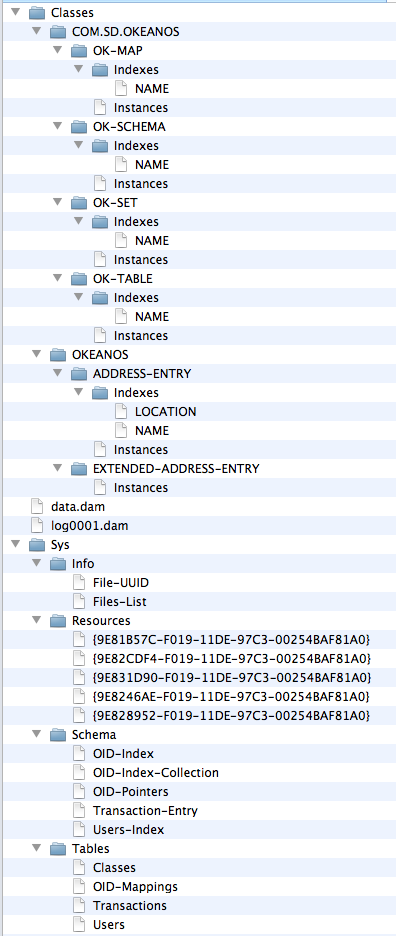
\includegraphics[width=3in]{OkeanosDatabaseFiles.png}
  \caption{Okeanos Database Files}
  \label{fig:OkeanosDatabaseFiles}
\end{figure}

The files named ``log0001.dam'' through ``log0004.dam'' in this picture are the transaction logs and object store for the database. All but the highest numbered file are treated as read-only repositories of past transaction logs and object data. The highest numbered file, ``log0004.dam'' in this case, contains the currently active transaction log and will be home to newly created persistent objects.

The file named ``data.dam'' contains the high-performance memory mapped B-Trees, heaps, and string-pool.

At the top of the picture you see the ``Classes'' folder, and inside of it are subfolders named after each Lisp package in which \texttt{PERSISTENT-OBJECT} subclasses were defined. Inside of each package folder is a collection of folders for every \texttt{PERSISTENT-OBJECT} class that ever had objects instantiated.  Within each of those class folders are the indexes and instance directories. Index files are named after the slots which are indexed. Index and instance directory files contain pointers to tables in the main B-Tree file, and those tables contain OID's to refer to instances in the main object repositories. As you can see, the OK-Schema and OK-Table classes are indexed by a Name slot. Those Name index files are the registries for their respective objects.

The ``Classes'' folder will grow over time with additional entries as new persistent subclasses get defined. Some of the class folders may have one or more index tables, and others may have none. This example shows very few in an effort to keep the presentation brief.

In the ``Sys'' folder we find Okeanos files that are used for its own internal purposes. The ``Sys/Info'' subfolder contains the database ID and the list of logfiles currently active. The ``Sys/Resources'' folder contains copies of schema that are tied directly to tables currently in use by Okeanos. The ``Sys/Schema'' folder contains schema files which hold images of their most recent versions.

The ``Sys/Tables'' folder has files which point to tables stored in the main memory-mapped ``data.dam'' file and that are used by Okeanos to manage the overall database. 

The ``OID-Mappings'' table is used to hold OID's, their timestamps, and pointers into the logfiles for the current copy of associated objects. 

The ``Transactions'' table holds TID's and file pointers into the transaction logs. That way we can quickly find any particular transaction and examine its logged entries.

All of these files should be considered READ-ONLY and hands-off. Okeanos manages them, and users should never try to modify them. None of them are human readable. We present this information solely to keep our users well informed.




\end{document}
%=%=%=%=%=%=%=%=%=%=%=%=%=%=%=%=%=%=%=%=%=%=%=%=%=%=%=%
